%% (Master) Thesis template
% Template version used: v1.4
%
% Largely adapted from Adrian Nievergelt's template for the ADPS
% (lecture notes) project.


%% We use the memoir class because it offers a many easy to use features.
\documentclass[11pt,a4paper,titlepage]{memoir}

%% Packages
%% ========

%% LaTeX Font encoding -- DO NOT CHANGE
\usepackage[OT1]{fontenc}

%% Babel provides support for languages.  'english' uses British
%% English hyphenation and text snippets like "Figure" and
%% "Theorem". Use the option 'ngerman' if your document is in German.
%% Use 'american' for American English.  Note that if you change this,
%% the next LaTeX run may show spurious errors.  Simply run it again.
%% If they persist, remove the .aux file and try again.
\usepackage[english]{babel}

%% Input encoding 'utf8'. In some cases you might need 'utf8x' for
%% extra symbols. Not all editors, especially on Windows, are UTF-8
%% capable, so you may want to use 'latin1' instead.
\usepackage[utf8]{inputenc}

%% This changes default fonts for both text and math mode to use Herman Zapfs
%% excellent Palatino font.  Do not change this.
\usepackage[sc]{mathpazo}

%% The AMS-LaTeX extensions for mathematical typesetting.  Do not
%% remove.
\usepackage{amsmath,amssymb,amsfonts,mathrsfs}

%% NTheorem is a reimplementation of the AMS Theorem package. This
%% will allow us to typeset theorems like examples, proofs and
%% similar.  Do not remove.
%% NOTE: Must be loaded AFTER amsmath, or the \qed placement will
%% break
\usepackage[amsmath,thmmarks]{ntheorem}

%% LaTeX' own graphics handling
\usepackage{graphicx}

%% We unfortunately need this for the Rules chapter.  Remove it
%% afterwards; or at least NEVER use its underlining features.
\usepackage{soul}

%% This allows you to add .pdf files. It is used to add the
%% declaration of originality.
\usepackage{pdfpages}

%% Some more packages that you may want to use.  Have a look at the
%% file, and consult the package docs for each.
%% See the TeXed file for more explanations

%% [OPT] Multi-rowed cells in tabulars
%\usepackage{multirow}

%% [REC] Intelligent cross reference package. This allows for nice
%% combined references that include the reference and a hint to where
%% to look for it.
\usepackage{varioref}

%% [OPT] Easily changeable quotes with \enquote{Text}
%\usepackage[german=swiss]{csquotes}

%% [REC] Format dates and time depending on locale
\usepackage{datetime}

%% [OPT] Provides a \cancel{} command to stroke through mathematics.
%\usepackage{cancel}

%% [NEED] This allows for additional typesetting tools in mathmode.
%% See its excellent documentation.
\usepackage{mathtools}

%% [NEED] Conditional commands
\usepackage{ifthen}

%% [OPT] Manual large braces or other delimiters.
%\usepackage{bigdelim, bigstrut}

%% [REC] Alternate vector arrows. Use the command \vv{} to get scaled
%% vector arrows.
\usepackage[h]{esvect}

%% [NEED] Some extensions to tabulars and array environments.
\usepackage{array}

%% [OPT] Postscript support via pstricks graphics package. Very
%% diverse applications.
%\usepackage{pstricks,pst-all}

%% [?] This seems to allow us to define some additional counters.
%\usepackage{etex}

%% [ADV] XY-Pic to typeset some matrix-style graphics
%\usepackage[all]{xy}

%% [OPT] This is needed to generate an index at the end of the
%% document.
%\usepackage{makeidx}

%% [OPT] Fancy package for source code listings.  The template text
%% needs it for some LaTeX snippets; remove/adapt the \lstset when you
%% remove the template content.
\usepackage{listings}
% \lstset{language=TeX,basicstyle={\normalfont\ttfamily}}

%% [REC] Fancy character protrusion.  Must be loaded after all fonts.
%\usepackage[activate]{pdfcprot}

%% [REC] Nicer tables.  Read the excellent documentation.
\usepackage{booktabs}

%% [OPT] Package for adding TODOs.
\usepackage{todonotes}

%% [OPT] Package to define and use acronyms
\usepackage[nolist,nohyperlinks,smaller]{acronym}
 

%% Our layout configuration.  DO NOT CHANGE.
%% Memoir layout setup

%% NOTE: You are strongly advised not to change any of them unless you
%% know what you are doing.  These settings strongly interact in the
%% final look of the document.

% Dependencies
\usepackage{ETHlogo}

% use helvetica as default font:
\usepackage[scaled]{helvet}
\renewcommand\familydefault{\sfdefault} 

% Turn extra space before chapter headings off.
\setlength{\beforechapskip}{0pt}

\nonzeroparskip
\parindent=0pt
\defaultlists

% Chapter style redefinition
\makeatletter

\makepagestyle{headerWPageNr}% Create headerWPageNr style
\if@twoside
  \copypagestyle{headerWPageNr}{Ruled}
  \copypagestyle{chapter}{Ruled}
\else
  \copypagestyle{headerWPageNr}{ruled}
  \copypagestyle{chapter}{ruled}
\fi
% chapter pages have no header and center page number in footer:
\makeoddhead{chapter}{}{}{}
\makeevenhead{chapter}{}{}{}
\makeoddfoot{chapter}{}{\thepage}{}
\makeevenfoot{chapter}{}{\thepage}{}
\makeheadrule{chapter}{\textwidth}{0pt}

% all other pages have page number and chapter or section name in header without footer:
\makeoddhead{headerWPageNr}{\rightmark}{}{\thepage}
\makeevenhead{headerWPageNr}{\thepage}{}{\leftmark}
\makeoddfoot{headerWPageNr}{}{}{}
\makeevenfoot{headerWPageNr}{}{}{}
\pagestyle{headerWPageNr}% Set page style to headerWPageNr


\makechapterstyle{bianchimod}{%
  \copypagestyle{abstract}{empty}
  \chapterstyle{default}
  \renewcommand*{\chapnamefont}{\normalfont\Large\sffamily}
  \renewcommand*{\chapnumfont}{\normalfont\Large\sffamily}
  \renewcommand*{\printchaptername}{%
    \chapnamefont\centering\@chapapp}
  \renewcommand*{\printchapternum}{\chapnumfont {\thechapter}}
  \renewcommand*{\chaptitlefont}{\normalfont\huge\sffamily}
  \renewcommand*{\printchaptertitle}[1]{%
    \hrule\vskip\onelineskip \centering \chaptitlefont\textbf{\vphantom{gyM}##1}\par}
  \renewcommand*{\afterchaptertitle}{\vskip\onelineskip \hrule\vskip
    \afterchapskip}
  \renewcommand*{\printchapternonum}{%
    \vphantom{\chapnumfont {9}}\afterchapternum}}
  
\makechapterstyle{bianchimod2}{%
  \renewenvironment{abstract}{\chapter*{\abstractname}}{}
  \chapterstyle{default}
  \definecolor{ChapGrey}{rgb}{0.6,0.6,0.6}
  \newcommand{\LargeFont}{% Needs a ’stretchable’ font
  	\usefont{\encodingdefault}{\sfdefault}{b}{n}%
    \fontsize{100}{0}\selectfont\color{ChapGrey}}
  \renewcommand*{\chapnumfont}{\LargeFont}
  \renewcommand*{\printchaptername}{\raggedleft}
  \renewcommand*{\printchapternum}{\chapnumfont {\thechapter}}
  \renewcommand*{\chaptitlefont}{\normalfont\Huge\sffamily\color{black}}
  \renewcommand*{\printchaptertitle}[1]{%
    \raggedleft \chaptitlefont\textbf{\vphantom{gyM}##1}\par}}

% Use the newly defined style
\chapterstyle{bianchimod}

\setsecheadstyle{\Large\bfseries\sffamily}
\setsubsecheadstyle{\large\bfseries\sffamily}
\setsubsubsecheadstyle{\bfseries\sffamily}
\setparaheadstyle{\normalsize\bfseries\sffamily}
\setsubparaheadstyle{\normalsize\itshape\sffamily}
\setsubparaindent{0pt}

% Set captions to a more separated style for clearness
\captionnamefont{\sffamily\bfseries\footnotesize}
\captiontitlefont{\sffamily\footnotesize}
\setlength{\intextsep}{16pt}
\setlength{\belowcaptionskip}{1pt}

% Set section and TOC numbering depth to subsection
\setsecnumdepth{subsection}
\settocdepth{subsection}

% definitions for titlepage
\def\@advisor{}
\newcommand{\advisor}[1]{\def\@advisor{#1}}
\def\@supervisor{}
\newcommand{\supervisor}[1]{\def\@supervisor{#1}}
\def\@group{}
\newcommand{\group}[1]{\def\@group{#1}}
\def\@institute{}
\newcommand{\institute}[1]{\def\@institute{#1}}
\def\@department{}
\newcommand{\department}[1]{\def\@department{#1}}
\def\@school{}
\newcommand{\school}[1]{\def\@school{#1}}
\def\@thesistype{}
\newcommand{\thesistype}[1]{\def\@thesistype{#1}}
\def\@email{}
\newcommand{\email}[1]{\def\@email{#1}}

%% Title page adjustments
% the following definition (either 0 or 1) controls the title page's layout:
\def\centeredtitlepage{1}
\if\centeredtitlepage1
	% default title page from cadmo template
	\newcommand{\maketitlepage}{
		\begin{titlingpage}
  			\calccentering{\unitlength}
  			\begin{adjustwidth*}{\unitlength-24pt}{-\unitlength-24pt}
    		\maketitle
  			\end{adjustwidth*}
		\end{titlingpage}
	}
	\pretitle{\vspace{0pt plus 0.7fill}\begin{center}\HUGE\sffamily\bfseries}
	\posttitle{\end{center}\par}
	\preauthor{\par\begin{center}\let\and\\\Large\sffamily}
	\postauthor{\end{center}}
	\predate{\par\begin{center}\Large\sffamily}
	\postdate{\end{center}}

	\renewcommand{\maketitlehooka}{\noindent\ETHlogo[2in]}

	\renewcommand{\maketitlehookb}{\vspace{1in}%
  		\par\begin{center}\Large\sffamily\@thesistype\end{center}}

	\renewcommand{\maketitlehookd}{%
  		\vfill\par
  			\begin{flushright}
    			\sffamily
    			Advisors: \@supervisor, \@advisor\par
    			\@department, \@school
  			\end{flushright}
	}

\else
	% alternative title page (right-aligned)
	\newcommand{\maketitlepage}{
		\begin{titlingpage}
			\titlestyleright
		\end{titlingpage}
	}
	\newcommand*\titlestyleright{
		\thispagestyle{empty}
		\sffamily
		\vspace*{\stretch{6}}
		\begin{flushright}
		{\Huge\sffamily\bfseries\@title}
		\par\noindent\rule[-1ex]{\linewidth}{2pt}\par
		\vspace{0.5cm}
		\emph{\huge\sffamily\@thesistype}
		\vspace{2cm}\par
		{\LARGE\sffamily\bfseries\@author}\par
		{\sffamily\@email}\par
		\vspace{1cm}
    	{\large\textbf{Advisor}\par
    		\@advisor\par}
    	\vspace{0.5cm}
    	{\large\textbf{Supervisor}\par
    		\@supervisor\par}
    	\vspace{1cm}
    	{\@group\par
    		\@institute\par
        	\@department\par
        	\@school\par}
    	\vspace{1cm}
    	{\normalsize\@date\par}
		\end{flushright}
		\vspace{\stretch{1}}
		\noindent\ETHlogo[2in]
		\pagebreak 
    	\sffamily
    	\thispagestyle{empty} 
	}
\fi

\checkandfixthelayout

\setlength{\droptitle}{-48pt}

\makeatother

% This defines how theorems should look. Best leave as is.
\theoremstyle{plain}
\setlength\theorempostskipamount{0pt}

%%% Local Variables:
%%% mode: latex
%%% TeX-master: "thesis"
%%% End:


%% Theorem environments.  You will have to adapt this for a German
%% thesis.
%% Theorem-like environments

%% This can be changed according to language. You can comment out the ones you
%% don't need.

\numberwithin{equation}{chapter}

%% German theorems
%\newtheorem{satz}{Satz}[chapter]
%\newtheorem{beispiel}[satz]{Beispiel}
%\newtheorem{bemerkung}[satz]{Bemerkung}
%\newtheorem{korrolar}[satz]{Korrolar}
%\newtheorem{definition}[satz]{Definition}
%\newtheorem{lemma}[satz]{Lemma}
%\newtheorem{proposition}[satz]{Proposition}

%% English variants
\newtheorem{theorem}{Theorem}[chapter]
\newtheorem{example}[theorem]{Example}
\newtheorem{remark}[theorem]{Remark}
\newtheorem{corollary}[theorem]{Corollary}
\newtheorem{definition}[theorem]{Definition}
\newtheorem{lemma}[theorem]{Lemma}
\newtheorem{proposition}[theorem]{Proposition}

%% Proof environment with a small square as a "qed" symbol
\theoremstyle{nonumberplain}
\theorembodyfont{\normalfont}
\theoremsymbol{\ensuremath{\square}}
\newtheorem{proof}{Proof}
%\newtheorem{beweis}{Beweis}


%% Helpful macros.
%% Custom commands
%% ===============

%% Special characters for number sets, e.g. real or complex numbers.
\newcommand{\C}{\mathbb{C}}
\newcommand{\K}{\mathbb{K}}
\newcommand{\N}{\mathbb{N}}
\newcommand{\Q}{\mathbb{Q}}
\newcommand{\R}{\mathbb{R}}
\newcommand{\Z}{\mathbb{Z}}
\newcommand{\X}{\mathbb{X}}

%% Fixed/scaling delimiter examples (see mathtools documentation)
\DeclarePairedDelimiter\abs{\lvert}{\rvert}
\DeclarePairedDelimiter\norm{\lVert}{\rVert}

%% Use the alternative epsilon per default and define the old one as \oldepsilon
\let\oldepsilon\epsilon
\renewcommand{\epsilon}{\ensuremath\varepsilon}

%% Also set the alternate phi as default.
\let\oldphi\phi
\renewcommand{\phi}{\ensuremath{\varphi}}


%% acronyms used in this thesis:
\begin{acronym}
\acro{WLAN}{Wireless LAN}
\acro{DCF}{Distributed Coordination Function}
\acro{AP}{Access Point}
\acro{IP}{Internet Protocol}
\acro{TCP}{Transmission Control Protocol}
\acro{UDP}{User Datagram Protocol}
\end{acronym}


%% Make document internal hyperlinks wherever possible. (TOC, references)
%% This MUST be loaded after varioref, which is loaded in 'extrapackages'
%% above.  We just load it last to be safe.
\usepackage[linkcolor=black,colorlinks=true,citecolor=black,filecolor=black]{hyperref}

%% Gobra environment
\usepackage{listings, silver}
\usepackage{color, colortbl}
\usepackage{xspace}
\usepackage{cite}
\usepackage{tikz}
\usepackage[colorlinks=true, urlcolor=blue]{hyperref}
\usepackage{hyphenat}
\usepackage[normalem]{ulem} %% Crossing out text (defines \sout)

\usepackage[inline]{enumitem} %% Provides inline lists, e.g. environment enumerate*
  \setlist*[enumerate]{label=(\arabic*)}

\usepackage{amsmath,amssymb,graphicx}
\usepackage{amsthm}
\usepackage{qsymbols}
\usepackage{stmaryrd} %% E.g. for \Mapsto
\usepackage{multirow}

\usepackage{suffix} %% Be able to declare starred macros, e.g. \foo*
\usepackage{xparse}
\usepackage[colorlinks=true, urlcolor=blue]{hyperref}

\newcommand*{\ListingsFontSize}{\fontsize{8.0}{8.3}\selectfont}
\newcommand*{\SilFont}{\ttfamily\ListingsFontSize}





% colors (see https://latexcolor.com/)
\definecolor{light-gray}{gray}{0.9}
\definecolor{darkgreen}{rgb}{0.0,0.7,0.0}
\definecolor{darkred}{rgb}{0.55, 0.0, 0.0}
\definecolor{persianblue}{rgb}{0.11, 0.22, 0.73}
\definecolor{navyblue}{rgb}{0.0, 0.0, 0.5}
\definecolor{darkpowderblue}{rgb}{0.0, 0.2, 0.6}
\definecolor{frenchblue}{rgb}{0.0, 0.45, 0.73}
\definecolor{burntorange}{rgb}{0.8, 0.33, 0.0}

\definecolor{rowShade}{gray}{0.85}



%% ****************************************************************************

\newcommand*{\Figref}[1]{Fig.~\ref{fig:#1}}
\newcommand*{\figref}{\Figref}
\newcommand*{\Secref}[1]{Sec.~\ref{sec:#1}}
\newcommand*{\secref}{\Secref}
\newcommand*{\Appref}[1]{App.~\ref{sec:#1}}
\newcommand*{\appref}{\Appref}
\newcommand*{\Lineref}[1]{Line~\ref{line:#1}}
\newcommand*{\lineref}[1]{line~\ref{line:#1}}
\newcommand*{\Linerange}[2]{Lines~\ref{line:#1}-\ref{line:#2}}
\newcommand*{\linerange}[2]{lines~\ref{line:#1}-\ref{line:#2}}
\newcommand*{\Sref}[1]{\hyperref[#1]{\S\ref*{#1}}}

%% ****************************************************************************

\newcommand*{\Ie}{I.e.\xspace}
\newcommand*{\ie}{i.e.\xspace}
\newcommand*{\Eg}{E.g.\xspace}
\newcommand*{\eg}{e.g.\xspace}
\newcommand*{\Cf}{Cf.\xspace}
\newcommand*{\cf}{cf.\xspace}
\newcommand*{\Wrt}{W.r.t.\xspace}
\newcommand*{\wrt}{w.r.t.\xspace}

\newcommand*{\naive}{na\"{\i}ve\xspace}
\newcommand*{\Naive}{Na\"{\i}ve\xspace}

%% ****************************************************************************

%% Convention: There are three macros per potential acronym, and a relation to
%% the \term macro defined further down, all of which to ensure that one can 
%% easily change if acronyms are used, and for which terms.
%% For example, for IVL:
%% - \IVL is the actual acronym ('{IVL}'), or it is simply empty ('{}').
%%   When a term is introduced that is (or may later be) used in acronym form,
%%   this should be done as follows:
%%     ... \term[\IVL]{intermediate verification language} ...
%%   This expands to 'intermediate verification language (IVL)', but if \IVL is empty,
%%   it expands to just 'intermediate verification language'.
%% - \Ivl and \ivl are intended to be used later on, after the term has been 
%%   introduced (via \term). Either both expand to the acronym ("IVL"), or
%%   \Ivl/\ivl expand to the full term, beginning with a capital/lower letter.

\newcommand*{\IVL}{IVL\xspace}
\newcommand*{\ivl}{intermediate verification language\xspace}
\newcommand*{\Ivl}{Intermediate verification language}

\newcommand*{\IIP}{IVL\xspace}
\newcommand*{\iip}{implementation proof\xspace}
\newcommand*{\Iip}{implementation proof}

\newcommand*{\termacronym}{}%
\NewDocumentCommand{\term}{O{} m}{%
  \textit{#2}%
  %% The first argument is expected to either be empty or to be an acronym.
  %% Empty can be: an omitted argument (\term{proof outline}), an explicitly
  %% provided by empty argument (\term[]{proof outline}) or a macro as an 
  %% argument that is defined as empty (\def\PO{} \term[\PO]{proof outline}).
  %% To cover all cases, several tests appear to be necessary.
  \renewcommand*{\termacronym}{}%
  \ifdefmacro{#1}{%
    %% Argument #1 is a macro. If not empty (void), we'll use it.
    \ifdefvoid{#1}{}{\renewcommand*{\termacronym}{#1}}%
  }{%
    %% Argument #1 is not a (defined) macro. If not empty (equal to {}),
    %% we'll use it.
    \ifthenelse{\equal{#1}{}}{}{\renewcommand*{\termacronym}{#1}}%
  }%
  \ifdefvoid{\termacronym}{}{ (\termacronym)}%
  \xspace%
}

%% ****************************************************************************

% \newcommand*{\ListingsFontSize}{\fontsize{8.0}{8.3}\selectfont}
% \newcommand*{\SilverFont}{\ttfamily\ListingsFontSize}
% \usepackage{silver}

%% listings
\lstset{numberstyle=\small} % size of line numbers
\lstset{mathescape=true}

\newcommand{\vcode}[1]{\vipercode{#1}}



% \lstset{
%   % basicstyle={\small\fontfamily{cmtt}\selectfont}
%   % basicstyle={\ttfamily\selectfont\footnotesize},
%   % commentstyle={\ttfamily\selectfont\footnotesize},
%   tabsize=2,
%   mathescape=true,
%   language=silver
%   % basicstyle=\ttfamily
% }

\newcommand*{\GobraFont}{\SilFont}
\newcommand*{\GobraFontSize}{\ListingsFontSize}
\newcommand*{\InlineGobraFontSize}{\small}

%% TODO: Add keywords (can we take them from Felix' thesis?)
\lstdefinelanguage{gobra}{
  language=go,
  sensitive=true,
  morecomment=[l]{//},
  morecomment=[s]{/*}{*/},
  morekeywords=[1]{ %% Keywords of the programming language subset
    pred, implements
  },
  morekeywords=[2]{ %% Keywords of the specification language subset
    requires, ensures, invariant, req, ens, pure
  },
  morekeywords=[3]{ %% Keywords of the proof language subset
    fold, unfold, unfolding, in, ghost,
    assume, assert, inhale, exhale
  },
  basicstyle={\GobraFont\GobraFontSize},
  commentstyle={\color[HTML]{747678}\textit},
  keywordstyle={[1]\color[HTML]{0005FF}},%\bfseries
  keywordstyle={[2]\color{burntorange}},%\bfseries
  keywordstyle={[3]\color[HTML]{EC008C}},%\bfseries
  mathescape=true,
  escapechar=§,
  moredelim=**[is][\normalfont\itshape]{'}{'} 
    %% Should use \var rather than \normalfont\itshape, but that doesn't work. 
    % Probably because \var expects an argument.
}

\lstdefinelanguage{myViper}{
  language=silver,
  sensitive=true,
  basicstyle={\GobraFont\GobraFontSize},
  mathescape=true,
  escapechar=§,
  moredelim=**[is][\normalfont\itshape]{'}{'} 
    %% Should use \var rather than \normalfont\itshape, but that doesn't work. 
    % Probably because \var expects an argument.
}

\lstdefinelanguage{plaintext}{
  language=,
  % basicstyle={\GobraFont\GobraFontSize},
  % commentstyle={\GobraFont\GobraFontSize\color{red}},
  keywordstyle=\bfseries,
  ndkeywordstyle=\bfseries,
  morecomment=[l]{//},
  mathescape=true
}

\makeatletter
\lst@Key{countblanklines}{true}[t]%
    {\lstKV@SetIf{#1}\lst@ifcountblanklines}

\lst@AddToHook{OnEmptyLine}{%
    \lst@ifnumberblanklines\else%
       \lst@ifcountblanklines\else%
         \advance\c@lstnumber-\@ne\relax%
       \fi%
    \fi}
\makeatother

\lstnewenvironment{gobra}[1][]{
  \lstset{
    language=gobra,
    floatplacement={tbp},
    captionpos=b,
    frame=lines,
    numbers=left,
    numberblanklines=false,
    xleftmargin=8pt,
    xrightmargin=8pt,
    countblanklines=false,
    numberstyle=\scriptsize,
    #1
  }
}{}


\lstnewenvironment{myViper}[1][]{
  \lstset{
    language=myViper,
    floatplacement={tbp},
    captionpos=b,
    frame=lines,
    numbers=left,
    numberblanklines=false,
    xleftmargin=8pt,
    xrightmargin=8pt,
    #1
  }
}{}

%% Use similar to \lstinline itself, e.g \gobra!x := a.f!, i.e. with a
%% surrounding delimiter.
%% http://tex.stackexchange.com/questions/100427/
\newcommand*{\inlgobra}{%
  \lstinline[%
    language=gobra,%
    columns=fixed,%
    basicstyle={\GobraFont\InlineGobraFontSize},%
    mathescape=true,%
    commentstyle={\color{black}\InlineGobraFontSize},
    keywordstyle={[1]\color{black}\InlineGobraFontSize},
    keywordstyle={[2]\color{black}\InlineGobraFontSize},
    keywordstyle={[3]\color{black}\InlineGobraFontSize},
    keywordstyle={[4]\color{black}\InlineGobraFontSize}
  ]%
}
\newcommand*{\gl}{\inlgobra}

\newcommand*{\inlmyviper}{%
  \lstinline[%
    language=myViper,%
    columns=fixed,%
    basicstyle={\GobraFont\InlineGobraFontSize},%
    commentstyle={\color{black}\InlineGobraFontSize},
    keywordstyle={[1]\color{black}\InlineGobraFontSize},
    keywordstyle={[2]\color{black}\InlineGobraFontSize},
    keywordstyle={[3]\color{black}\InlineGobraFontSize},
    keywordstyle={[4]\color{black}\InlineGobraFontSize}
  ]%
}
\newcommand*{\vl}{\inlmyviper}

%% Ensure that \texttt and \inlgobra use the same font in the same size.
%% Important, because it is sometimes seemingly impossible to use \inlgobra 
%% (in general, verbatim text) in certain situations, in which case one can
%% fallback to \texttt.
\usepackage{letltxmacro} %% Provides \LetLtxMacro
\LetLtxMacro\oldttfamily\ttfamily
\DeclareRobustCommand{\ttfamily}{\oldttfamily\InlineGobraFontSize}

%% ****************************************************************************

% Encoding

\newcommand{\encodeT}[1]{\llbracket #1 \rrbracket}
\newcommand{\shared}[0]{@}
\newcommand{\exclusive}[0]{\bullet}
\newcommand{\encAs}[0]{\triangleq}

\newcommand{\implementationProof}{_{\textsc{Proof}}}


%% Document information
%% ====================

\title{Secure Deletion of Sensitive Data in Protocol Implementations}
\author{Hugo Queinnec}
\email{hqueinnec@student.ethz.ch}
\thesistype{Master's Thesis}
\advisor{Linard Arquint}
\supervisor{Prof.\ Dr.\ Peter Müller}
\group{Programming Methodology}
\institute{Institute for Programming Languages and Systems}
\department{Department of Computer Science}
\school{ETH Z\"urich}
\date{September 24, 2023}

\begin{document}

\frontmatter

%% Title page is autogenerated from document information above.  DO
%% NOT CHANGE.
\maketitlepage

%% The abstract of your thesis.  Edit the file as needed.
\begin{abstract}
  This example thesis briefly shows the main features of our thesis
  style, and how to use it for your purposes.
  \todo[inline]{Change abstract}
\end{abstract}


%% reset acronym usage:
\acresetall

%% TOC with the proper setup, do not change.
\cleartorecto
\tableofcontents
\mainmatter

%% Your real content!
% \chapter{Introduction}
\label{chap:introduction}

% 1. Security protocols are ubiquitous (everywhere)
% 2. Protocols and their implementation should be correct because high stakes are at risk (banking)
% 3. We need to guarantee security properties: it is not easy (worst case, infinity of executions)
% 4. Lots of research on protocol verification, but we also need guarantees for implementations
% 5. While [authors + citation] propose a promising methodology for verifying security properties for protocol implementations, they cannot reason about sensitive data that must be deleted in a timely manner. This is crucial for proving strong security properties such as post-compromise security.

Security protocols are omnipresent in our daily lives, they are the foundation for many applications ranging from online banking to text messaging. These protocols employ cryptography to achieve fundamental security properties such as authentication and confidentiality.
Online banking operations serve as a prime example of how heavily we rely on security protocols. A breach in the security of these protocols could lead to substantial financial losses, which is why it is essential that these protocols and their implementations are both correct and secure.
% For example, proving a property such as \emph{injective agreement} protects against replay attacks and prevents a transaction from being repeated multiple times.
For example, proving a property such as \emph{injective agreement} protects against replay attacks, meaning that the protocol participants reject messages from an attacker attempting to resend messages that participants may have sent in the past. In our online banking example, such a message could contain the request to perform a certain transaction, and it is thus crucial that this request cannot be replayed by an attacker.

Moreover, security protocols are not limited to the banking sector and are now crucial to a wider audience, especially for secure messaging.
Secure messaging is a cornerstone of modern communication, with individuals, businesses, and governments relying on it to protect sensitive information.
Robust security protocols are paramount in safeguarding the confidentiality and integrity of messages.
For instance, a security breach could lead to the exposure of personal conversations, critical business data, or confidential government communications, potentially resulting in severe consequences.
Therefore, several popular messaging applications, such as Signal, WhatsApp, and Facebook Messenger, rely on the Signal protocol \cite{} to offer secure and end-to-end encrypted communication to billions of users.

Guaranteeing security properties for protocols is a challenging task, especially in the presence of a strong attacker.
In order to ensure these properties for all possible protocol executions, verification must consider an arbitrary number of participants and protocol sessions, as well as any possible ordering of protocol steps. Furthermore, protocol security properties are generally not local to a particular participant but global, such as mutual authentication between two parties. This presents an additional challenge for verification as it requires a global view of the protocol execution.
Moreover, it is also particularly difficult to reason about implementation-level specificities, such as mutable state and concurrency, while reasoning about security properties.

In this regard, two aspects of the protocol must be considered: the high-level protocol itself (that we will call \emph{model}), and its implementation. Proving security properties for a protocol model is an active field of research and several promising automatic verifiers have been proposed (like Tamarin \cite{}). However, a verified protocol model does not imply that an implementation is free of security vulnerabilities and achieves the same security properties as its model. This is why we focus on verifying security properties for protocol implementations.

While Arquint and al.\cite{} propose a promising methodology for verifying security properties for protocol implementations, they do not reason about sensitive data that must be deleted in a timely manner.
However, such reasoning is necessary for proving security properties like forward secrecy and post-compromise security, for protocols that periodically renew keys, like Signal \cite{}.
% Forward secrecy guarantees that an attacker cannot compute the session keys of an already established session after learning the long-term secret keys.
Forward secrecy informally guarantees that past keys remain secret even when newer keys or long-term keys become known to the attacker.
It is crucial for secure communication, as it ensures that an attacker cannot decrypt past messages even if they manage to compromise a participant later on.
Post-compromise security informally means that a participant can communicate securely with a peer, even when certain secrets from the past have leaked.
%even if the peer’s secrets have already been (partly) compromised \cite{}.
This is sometimes referred to as \emph{healing}, which allows communication to resume securely at some point after a compromise.
Protocols like Signal achieve both of these properties by using a key rotation scheme within a protocol session, where a communication key is used to generate its successor and is then deleted.

The work of Arquint et al. comes with a Reusable Verification Library that implements protocol-independent components of the methodology to reduce the verification effort per protocol.
Because their methodology is generic, the Reusable Verification Library can be implemented in a wide variety of programming languages.
For the scope of this thesis, we will limit ourselves to protocol implementations written in Go, for which the Reusable Verification Library has been implemented.

In this thesis, we extend the methodology for the modular verification of security protocol implementations by Arquint et al. to make it capable of reasoning about sensitive and ephemeral data that must exist only for a limited time before being deleted.
We present a generic extension of the methodology that allows the verification of any type of protocol implementation using ephemeral data, like Signal, in order to satisfy strong security properties such as forward secrecy and post-compromise security.
In addition to the methodology, we extend the Go Reusable Verification Library accordingly.
Finally, we evaluate our methodology and our extension of the Go Reusable Verification Library by partly verifying a protocol implementation employing a key rotation scheme to achieve forward secrecy and post-compromise security.


\section{Outline}
\label{sec:outline}
% Clearly mention that the case study represents the evaluation of our methodology

The remainder of this thesis proceeds as follows.

In Chapter \ref{chap:background}, we introduce the necessary background knowledge for this thesis, including an introduction to the verification of Go programs, a review of existing works aiming at verifying protocol implementations, and explanations of basic cryptography concepts.

In Chapter \ref{chap:design}, we first present the conceptual idea behind our methodology to verify protocol implementations relying on ephemeral data. We then explain how we extended the Go Reusable Verification Library to support our methodology.

In Chapter \ref{chap:case-study}, we present a case study of our methodology on a Signal-like protocol implementation, and explain how we can use the library to verify strong security properties for this implementation.

Finally, in Chapter \ref{chap:conclusion}, we conclude and discuss future work.

% \chapter{Writing scientific texts in English}

This chapter was originally a separate document written by Reto
Spöhel.  It is reprinted here so that the template can serve as a
quick guide to thesis writing, and to provide some more example
material to give you a feeling for good typesetting.

% We're going to need an extra theorem-like environment for this
% chapter
\theoremstyle{plain}
\theoremsymbol{}
\newtheorem{Rule}[theorem]{Rule}

\section{Basic writing rules}

The following rules need little further explanation; they are best
understood by looking at the example in the booklet by Knuth et al.,
§2--§3.

\begin{Rule}
  Write texts, not chains of formulas.
\end{Rule}

More specifically, write full sentences that are logically
interconnected by phrases like `Therefore', `However', `On the other
hand', etc.\ where appropriate.

\begin{Rule}
  Displayed formulas should be embedded in your text and punctuated
  with it.
\end{Rule}

In other words, your writing should not be divided into `text parts'
and `formula parts'; instead the formulas should be tied together by
your prose such that there is a natural flow to your writing.

\section{Being nice to the reader}

Try to write your text in such a way that a reader enjoys reading
it. That's of course a lofty goal, but nevertheless one you should
aspire to!

\begin{Rule}
  Be nice to the reader.
\end{Rule}

Give some intuition or easy example for definitions and theorems which
might be hard to digest. Remind the reader of notations you introduced
many pages ago -- chances are he has forgotten them. Illustrate your
writing with diagrams and pictures where this helps the reader. Etc.

\begin{Rule}
  Organize your writing.
\end{Rule}

Think carefully about how you subdivide your thesis into chapters,
sections, and possibly subsections.  Give overviews at the beginning
of your thesis and of each chapter, so the reader knows what to
expect. In proofs, outline the main ideas before going into technical
details. Give the reader the opportunity to `catch up with you' by
summing up your findings periodically.

\emph{Useful phrases:} `So far we have shown that \ldots', `It remains
to show that \ldots', `Recall that we want to prove inequality (7), as
this will allow us to deduce that \ldots', `Thus we can conclude that
\ldots. Next, we would like to find out whether \ldots', etc.

\begin{Rule}
  Don't say the same thing twice without telling the reader that you
  are saying it twice.
\end{Rule}

Repetition of key ideas is important and helpful. However, if you
present the same idea, definition or observation twice (in the same or
different words) without telling the reader, he will be looking for
something new where there is nothing new.

\emph{Useful phrases:} `Recall that [we have seen in Chapter 5 that]
\ldots', `As argued before / in the proof of Lemma 3, \ldots', `As
mentioned in the introduction, \ldots', `In other words, \ldots', etc.

\begin{Rule}
  Don't make statements that you will justify later without telling
  the reader that you will justify them later.
\end{Rule}

This rule also applies when the justification is coming right in the
next sentence!  The reasoning should be clear: if you violate it, the
reader will lose valuable time trying to figure out on his own what
you were going to explain to him anyway.

\emph{Useful phrases:} `Next we argue that \ldots', `As we shall see,
\ldots', `We will see in the next section that \ldots, etc.


\section{A few important grammar rules}

\begin{Rule}
  \label{rule:no-comma-before-that}
  There is (almost) \emph{never} a comma before `that'.
\end{Rule}

It's really that simple. Examples:
\begin{quote}
  We assume that \ldots\\
  \emph{Wir nehmen an, dass \ldots}

  It follows that \ldots\\
  \emph{Daraus folgt, dass \ldots}

  `thrice' is a word that is seldom used.\\
  \emph{`thrice' ist ein Wort, das selten verwendet wird.}
\end{quote}
Exceptions to this rule are rare and usually pretty obvious. For
example, you may end up with a comma before `that' because `i.e.' is
spelled out as `that is':
\begin{quote}
  For \(p(n)=\log n/n\) we have \ldots{} However, if we choose \(p\) a
  little bit higher, that is \(p(n)=(1+\varepsilon)\log n/n\) for some
  \(\varepsilon>0\), we obtain that\ldots
\end{quote}
Or you may get a comma before `that' because there is some additional
information inserted in the middle of your sentence:
\begin{quote}
  Thus we found a number, namely \(n_0\), that satisfies equation (13).
\end{quote}
If the additional information is left out, the sentence has no comma:
\begin{quote}
  Thus we found a number that satisfies equation (13).
\end{quote}
(For `that' as a relative pronoun, see also
Rules~\ref{rule:non-defining-has-comma}
and~\ref{rule:defining-without-comma} below.)

\begin{Rule}
  There is usually no comma before `if'.
\end{Rule}

Example:
\begin{quote}
  A graph is not \(3\)-colorable if it contains a \(4\)-clique.\\
  \emph{Ein Graph ist nicht \(3\)-färbbar, wenn er eine \(4\)-Clique
    enthält.}
\end{quote}
However, if the `if' clause comes first, it is usually separated from
the main clause by a comma:
\begin{quote}
  If a graph contains a \(4\)-clique, it is not \(3\)-colorable .\\
  \emph{Wenn ein Graph eine \(4\)-Clique enthält, ist er nicht
    \(3\)-färbbar.}
\end{quote}

There are more exceptions to these rules than to
Rule~\ref{rule:no-comma-before-that}, which is why we are not
discussing them here. Just keep in mind: don't put a comma before `if'
without good reason.

\begin{Rule}
  \label{rule:non-defining-has-comma}
  Non-defining relative clauses have commas.
\end{Rule}
\begin{Rule}
  \label{rule:defining-without-comma}
  Defining relative clauses have no commas.
\end{Rule}

In English, it is very important to distinguish between two types of
relative clauses: defining and non-defining ones. This is a
distinction you absolutely need to understand to write scientific
texts, because mistakes in this area actually distort the meaning of
your text!

It's probably easier to explain first what a \emph{non-defining}
relative clause is. A non-defining relative clauses simply gives
additional information \emph{that could also be left out} (or given in
a separate sentence). For example, the sentence
\begin{quote}
  The \textsc{WeirdSort} algorithm, which was found by the famous
  mathematician John Doe, is theoretically best possible but difficult
  to implement in practice.
\end{quote}
would be fully understandable if the relative clause were left out
completely. It could also be rephrased as two separate sentences:
\begin{quote}
  The \textsc{WeirdSort} algorithm is theoretically best possible but
  difficult to implement in practice. [By the way,] \textsc{WeirdSort}
  was found by the famous mathematician John Doe.
\end{quote}
This is what a non-defining relative clause is. \emph{Non-defining
  relative clauses are always written with commas.} As a corollary we
obtain that you cannot use `that' in non-defining relative clauses
(see Rule~\ref{rule:no-comma-before-that}!). It would be wrong to
write
\begin{quote}
  \st{The \textsc{WeirdSort} algorithm, that was found by the famous
    mathematician John Doe, is theoretically best possible but
    difficult to implement in practice.}
\end{quote}
A special case that warrants its own example is when `which' is
referring to the entire preceding sentence:
\begin{quote}
  Thus inequality (7) is true, which implies that the Riemann
  hypothesis holds.
\end{quote}
As before, this is a non-defining relative sentence (it could be left
out) and therefore needs a comma.

So let's discuss \emph{defining} relative clauses next. A defining
relative clause tells the reader \emph{which specific item the main
  clause is talking about}. Leaving it out either changes the meaning
of the sentence or renders it incomprehensible altogether.  Consider
the following example:

\begin{quote}
  The \textsc{WeirdSort} algorithm is difficult to implement in
  practice. In contrast, the algorithm that we suggest is very simple.
\end{quote}

Here the relative clause `that we suggest' cannot be left out -- the
remaining sentence would make no sense since the reader would not know
which algorithm it is talking about. This is what a defining relative
clause is. \textit{Defining relative clauses are never written with
  commas.} Usually, you can use both `that' and `which' in defining
relative clauses, although in many cases `that' sounds better.

As a final example, consider the following sentence:
\begin{quote}
  For the elements in \(\mathcal{B}\) which satisfy property (A), we
  know that equation (37) holds.
\end{quote}
This sentence does not make a statement about all elements in
\(\mathcal{B}\), only about those satisfying property (A). The relative
clause is \emph{defining}. (Thus we could also use `that' in place of
`which'.)

In contrast, if we add a comma the sentence reads
\begin{quote}
  For the elements in \(\mathcal{B}\), which satisfy property (A), we
  know that equation (37) holds.
\end{quote}

Now the relative clause is \emph{non-defining} -- it just mentions in
passing that all elements in \(\mathcal{B}\) satisfy property (A). The
main clause states that equation (37) holds for \emph{all} elements in
\(\mathcal{B}\). See the difference?


\section[Things you (usually) don't say in English]%
{Things you (usually) don't say in English -- and what to say
  instead}
\label{sec:list}

Table~\ref{tab:things-you-dont-say} lists some common mistakes and
alternatives.  The entries should not be taken as gospel -- they don't
necessarily mean that a given word or formulation is wrong under all
circumstances (obviously, this depends a lot on the context). However,
in nine out of ten instances the suggested alternative is the better
word to use.

\begin{table}
  \centering
  \caption{Things you (usually) don't say}
  \label{tab:things-you-dont-say}
  \begin{tabular}{lll}
    \toprule
    \st{It holds (that) \dots} & We have \dots & \emph{Es gilt \dots}\\
    \multicolumn{3}{l}{\quad\footnotesize(`Equation (5) holds.' is fine, though.)}\\
    \st{$x$ fulfills property $\mathcal{P}$.}& \(x\) satisfies property \(\mathcal{P}\). & \emph{\(x\) erfüllt Eigenschaft \(\mathcal{P}\).} \\
    \st{in average} & on average & \emph{im Durchschnitt}\\
    \st{estimation} & estimate   & \emph{Abschätzung}\\
    \st{composed number} & composite number & \emph{zusammengesetzte Zahl}\\
    \st{with the help of} & using & \emph{mit Hilfe von}\\
    \st{surely} & clearly & \emph{sicher, bestimmt}\\
    \st{monotonously increasing} & monotonically incr. & \emph{monoton steigend}\\
    \multicolumn{3}{l}{\quad\footnotesize(Actually, in most cases `increasing' is just fine.)}\\
    \bottomrule
  \end{tabular}
\end{table}

%%% Local Variables:
%%% mode: latex
%%% TeX-master: "thesis"
%%% End:

% \chapter{Typography}


\section{Punctuation}

\begin{Rule}
  Use opening (`) and closing (') quotation marks correctly.
\end{Rule}

In \LaTeX, the closing quotation mark is typed like a normal
apostrophe, while the opening quotation mark is typed using the French
\emph{accent grave} on your keyboard (the \emph{accent grave} is the
one going down, as in \emph{frère}).

Note that any punctuation that \emph{semantically} follows quoted
speech goes inside the quotes in American English, but outside in
Britain.  Also, Americans use double quotes first.  Oppose
\begin{quote}
  ``Using `lasers,' we punch a hole in \ldots\ the Ozone Layer,''
  Dr.\ Evil said.
\end{quote}
to
\begin{quote}
  `Using ``lasers'', we punch a hole in \ldots\ the Ozone Layer',
  Dr.\ Evil said.
\end{quote}

\begin{Rule}
  Use hyphens (-), en-dashes (--) and em-dashes (---) correctly.
\end{Rule}

A hyphen is only used in words like `well-known', `$3$-colorable'
etc., or to separate words that continue in the next line (which is
known as hyphenation).  It is entered as a single ASCII hyphen
character (\texttt{-}).

To denote ranges of numbers, chapters, etc., use an en-dash (entered
as two ASCII hyphens \texttt{--}) with no spaces on either side.  For
example, using Equations (1)--(3), we see\ldots

As the equivalent of the German \emph{Gedankenstrich}, use an en-dash
with spaces on both sides -- in the title of Section \ref{sec:list},
it would be wrong to use a hyphen instead of the dash. (Some English
authors use the even longer emdash (---) instead, which is typed as
three subsequent hyphens in \LaTeX. This emdash is used without spaces
around it---like so.)


\section{Spacing}

\begin{Rule}
  \label{rule:no-manual-spacing}
  Do not add spacing manually.
\end{Rule}

You should never use the commands \lstinline-\\- (except within
tabulars and arrays), \lstinline[showspaces=true]-\ - (except to
prevent a sentence-ending space after Dr.\ and such),
\lstinline-\vspace-, \lstinline-\hspace-, etc.  The choices programmed
into \LaTeX{} and this style should cover almost all cases.  Doing it
manually quickly leads to inconsistent spacing, which looks terrible.
Note that this list of commands is by no means conclusive.

\begin{Rule}
  Judiciously insert spacing in maths where it helps.
\end{Rule}

This directly contradicts Rule~\ref{rule:no-manual-spacing}, but in
some cases \TeX{} fails to correctly decide how much spacing is
required.  For example, consider
\begin{displaymath}
  f(a,b) = f(a+b, a-b).
\end{displaymath}
In such cases, inserting a thin math space \lstinline-\,- greatly
increases readability:
\begin{displaymath}
  f(a,b) = f(a+b,\, a-b).
\end{displaymath}

Along similar lines, there are variations of some symbols with
different spacing.  For example, Lagrange's Theorem states that
\(\abs{G}=[G:H]\abs{H}\), but the proof uses a bijection \(f\colon
aH\to bH\).  (Note how the first colon is symmetrically spaced, but
the second is not.)

\begin{Rule}
  Learn when to use \lstinline[showspaces=true]-\ - and
  \lstinline-\@-.
\end{Rule}

Unless you use `french spacing', the space at the end of a sentence is
slightly larger than the normal interword space.

The rule used by \TeX{} is that any space following a period,
exclamation mark or question mark is sentence-ending, except for
periods preceded by an upper-case letter.  Inserting \lstinline-\-
before a space turns it into an interword space, and inserting
\lstinline-\@- before a period makes it sentence-ending.  This means
you should write
\begin{lstlisting}
Prof.\ Dr.\ A. Steger is a member of CADMO\@.
If you want to write a thesis with her, you
should use this template.
\end{lstlisting}
which turns into
\begin{quote}
  Prof.\ Dr.\ A. Steger is a member of CADMO\@.  If you want to write
  a thesis with her, you should use this template.
\end{quote}
The effect becomes more dramatic in lines that are stretched slightly
during justification:
\begin{quote}
  \parbox{\linewidth}{\hbox to \linewidth{%
      Prof.\ Dr.\ A. Steger is a member of CADMO\@.  If you}}
\end{quote}

\begin{Rule}
  Place a non-breaking space (\lstinline-~-) right before references.
\end{Rule}

This is actually a slight simplification of the real rule, which
should invoke common sense.  Place non-breaking spaces where a line
break would look `funny' because it occurs right in the middle of a
construction, especially between a reference type (Chapter) and its
number.


\section{Choice of `fonts'}

Professional typography distinguishes many font attributes, such as
family, size, shape, and weight.  The choice for sectional divisions
and layout elements has been made, but you will still occasionally
want to switch to something else to get the reader's attention.  The
most important rule is very simple.

\begin{Rule}
  When emphasising a short bit of text, use \lstinline-\emph-.
\end{Rule}

In particular, \emph{never} use bold text (\lstinline-\textbf-).
Italics (or Roman type if used within italics) avoids distracting the
eye with the huge blobs of ink in the middle of the text that bold
text so quickly introduces.

Occasionally you will need more notation, for example, a consistent
typeface used to identify algorithms.

\begin{Rule}
  Vary one attribute at a time.
\end{Rule}

For example, for \textsc{WeirdSort} we only changed the shape to small
caps.  Changing two attributes, say, to bold small caps would be
excessive (\LaTeX{} does not even have this particular variation).
The same holds for mathematical notation: the reader can easily
distinguish \(g_n\), \(G(x)\), \(\mathcal{G}\) and \(\mathsf{G}\).

\begin{Rule}
  Never underline or uppercase.
\end{Rule}

No exceptions to this one, unless you are writing your thesis on a
typewriter.  Manually.  Uphill both ways.  In a blizzard.


\section{Displayed equations}

\begin{Rule}
  Insert paragraph breaks \emph{after} displays only where they
  belong.  Never insert paragraph breaks \emph{before} displays.
\end{Rule}

\LaTeX{} translates sequences of more than one linebreak (i.e., what
looks like an empty line in the source code) into a paragraph break in
almost all contexts.  This also happens before and after displays,
where extra spacing is inserted to give a visual indication of the
structure.  Adding a blank line in these places may look nice in the
sources, but compare the resulting display

\begin{displaymath}
  a = b
\end{displaymath}

to the following:
\begin{displaymath}
  a = b
\end{displaymath}
The first display is surrounded by blank lines, but the second is not.
It is bad style to start a paragraph with a display (you should always
tell the reader what the display means first), so the rule follows.

\begin{Rule}
  Never use \lstinline-eqnarray-.
\end{Rule}

It is at the root of most ill-spaced multiline displays.  The
\package{amsmath} package provides better alternatives, such as the
\lstinline-align- family
\begin{align*}
  f(x) &= \sin x, \\
  g(x) &= \cos x,
\end{align*}
and \lstinline-multline- which copes with excessively long equations:
\begin{multline*}
  \def\P{\mathrm P}
  \P\bigl[X_{t_0} \in (z_0, z_0+dz_0],\ldots, X_{t_n}\in(z_n,z_n+dz_n]\bigr]
  \\= \nu(dz_0) K_{t_1}(z_0,dz_1) K_{t_2-t_1}(z_1,dz_2)\cdots
  K_{t_n-t_{n-1}}(z_{n-1},dz_n).
\end{multline*}


\section{Floats}

By default this style provides floating environments for tables and
figures.  The general structure should be as follows:
\begin{lstlisting}
\begin{figure}
  \centering
  % content goes here
  \caption{A short caption}
  \label{some-short-label}
\end{figure}
\end{lstlisting}
Note that the label must follow the caption, otherwise the label will
refer to the surrounding section instead.  Also note that figures
should be captioned at the bottom, and tables at the top.

The whole point of floats is that they, well, \emph{float} to a place
where they fit without interrupting the text body.  This is a frequent
source of confusion and changes; please leave it as is.

\begin{Rule}
  Do not restrict float movement to only `here'
  \textnormal{(\lstinline-h-)}.
\end{Rule}

If you are still tempted, you should avoid the float altogether and
just show the figure or table inline, similar to a displayed equation.

%%% Local Variables:
%%% mode: latex
%%% TeX-master: "thesis"
%%% End:

% \chapter{Example Chapter}

Dummy text. First use of an acronym: \ac{UDP}. Only short-hand of acronym is used when it reappears: \ac{UDP}.

Some Gobra and Viper code can be seen in figure~\ref{lst:echoServer} and~\ref{lst:silver_fields}, respectively.

\begin{figure}
  \begin{gobra}
    class Server(Thread):
      def run():
        server_socket = create_server_socket()
        while True:
          client_socket = server_socket.accept()
          data = client_socket.read_all(timeout=1)
          if data:
            print(client_socket.address)
            client_socket.send(data)
          client_socket.close()
  \end{gobra}
  \caption{Echo server.}
  \label{lst:echoServer}
\end{figure}

\begin{figure}
    \begin{myViper}
      field f: Int
      field g: Int
      method get_f(arg: Ref) returns (res1: Int,
                                      res2: Int)
        requires acc(arg.f)
        ensures acc(arg.f) && res1 == arg.f
      {
        res1 := arg.f
      //res2 := arg.g   // Verification error: might
                        // not have permission to
                        // access arg.g.
      }
    \end{myViper}
    \caption{A simple getter method. The assignment to the result
        variable \vl+res2+ fails to verify because the method does
        not have a permission to access field \vl+arg.g+.}
    \label{lst:silver_fields}
\end{figure}


\section{Example Section}

Dummy text.

\subsection{Example Subsection}

Dummy text.

\subsubsection{Example Subsubsection}

Dummy text.

\paragraph{Example Paragraph}

Dummy text.

\subparagraph{Example Subparagraph}

Dummy text. 

\chapter{Introduction}
\label{chap:introduction}

% 1. Security protocols are ubiquitous (everywhere)
% 2. Protocols and their implementation should be correct because high stakes are at risk (banking)
% 3. We need to guarantee security properties: it is not easy (worst case, infinity of executions)
% 4. Lots of research on protocol verification, but we also need guarantees for implementations
% 5. While [authors + citation] propose a promising methodology for verifying security properties for protocol implementations, they cannot reason about sensitive data that must be deleted in a timely manner. This is crucial for proving strong security properties such as post-compromise security.

Security protocols are omnipresent in our daily lives, they are the foundation for many applications ranging from online banking to text messaging. These protocols employ cryptography to achieve fundamental security properties such as authentication and confidentiality.
Online banking operations serve as a prime example of how heavily we rely on security protocols. A breach in the security of these protocols could lead to substantial financial losses, which is why it is essential that these protocols and their implementations are both correct and secure.
% For example, proving a property such as \emph{injective agreement} protects against replay attacks and prevents a transaction from being repeated multiple times.
For example, proving a property such as \emph{injective agreement} protects against replay attacks, meaning that the protocol participants reject messages from an attacker attempting to resend messages that participants may have sent in the past. In our online banking example, such a message could contain the request to perform a certain transaction, and it is thus crucial that this request cannot be replayed by an attacker.

Moreover, security protocols are not limited to the banking sector and are now crucial to a wider audience, especially for secure messaging.
Secure messaging is a cornerstone of modern communication, with individuals, businesses, and governments relying on it to protect sensitive information.
Robust security protocols are paramount in safeguarding the confidentiality and integrity of messages.
For instance, a security breach could lead to the exposure of personal conversations, critical business data, or confidential government communications, potentially resulting in severe consequences.
Therefore, several popular messaging applications, such as Signal, WhatsApp, and Facebook Messenger, rely on the Signal protocol \cite{} to offer secure and end-to-end encrypted communication to billions of users.

Guaranteeing security properties for protocols is a challenging task, especially in the presence of a strong attacker.
In order to ensure these properties for all possible protocol executions, verification must consider an arbitrary number of participants and protocol sessions, as well as any possible ordering of protocol steps. Furthermore, protocol security properties are generally not local to a particular participant but global, such as mutual authentication between two parties. This presents an additional challenge for verification as it requires a global view of the protocol execution.
Moreover, it is also particularly difficult to reason about implementation-level specificities, such as mutable state and concurrency, while reasoning about security properties.

In this regard, two aspects of the protocol must be considered: the high-level protocol itself (that we will call \emph{model}), and its implementation. Proving security properties for a protocol model is an active field of research and several promising automatic verifiers have been proposed (like Tamarin \cite{}). However, a verified protocol model does not imply that an implementation is free of security vulnerabilities and achieves the same security properties as its model. This is why we focus on verifying security properties for protocol implementations.

While Arquint and al.\cite{} propose a promising methodology for verifying security properties for protocol implementations, they do not reason about sensitive data that must be deleted in a timely manner.
However, such reasoning is necessary for proving security properties like forward secrecy and post-compromise security, for protocols that periodically renew keys, like Signal \cite{}.
% Forward secrecy guarantees that an attacker cannot compute the session keys of an already established session after learning the long-term secret keys.
Forward secrecy informally guarantees that past keys remain secret even when newer keys or long-term keys become known to the attacker.
It is crucial for secure communication, as it ensures that an attacker cannot decrypt past messages even if they manage to compromise a participant later on.
Post-compromise security informally means that a participant can communicate securely with a peer, even when certain secrets from the past have leaked.
%even if the peer’s secrets have already been (partly) compromised \cite{}.
This is sometimes referred to as \emph{healing}, which allows communication to resume securely at some point after a compromise.
Protocols like Signal achieve both of these properties by using a key rotation scheme within a protocol session, where a communication key is used to generate its successor and is then deleted.

The work of Arquint et al. comes with a Reusable Verification Library that implements protocol-independent components of the methodology to reduce the verification effort per protocol.
Because their methodology is generic, the Reusable Verification Library can be implemented in a wide variety of programming languages.
For the scope of this thesis, we will limit ourselves to protocol implementations written in Go, for which the Reusable Verification Library has been implemented.

In this thesis, we extend the methodology for the modular verification of security protocol implementations by Arquint et al. to make it capable of reasoning about sensitive and ephemeral data that must exist only for a limited time before being deleted.
We present a generic extension of the methodology that allows the verification of any type of protocol implementation using ephemeral data, like Signal, in order to satisfy strong security properties such as forward secrecy and post-compromise security.
In addition to the methodology, we extend the Go Reusable Verification Library accordingly.
Finally, we evaluate our methodology and our extension of the Go Reusable Verification Library by partly verifying a protocol implementation employing a key rotation scheme to achieve forward secrecy and post-compromise security.


\section{Outline}
\label{sec:outline}
% Clearly mention that the case study represents the evaluation of our methodology

The remainder of this thesis proceeds as follows.

In Chapter \ref{chap:background}, we introduce the necessary background knowledge for this thesis, including an introduction to the verification of Go programs, a review of existing works aiming at verifying protocol implementations, and explanations of basic cryptography concepts.

In Chapter \ref{chap:design}, we first present the conceptual idea behind our methodology to verify protocol implementations relying on ephemeral data. We then explain how we extended the Go Reusable Verification Library to support our methodology.

In Chapter \ref{chap:case-study}, we present a case study of our methodology on a Signal-like protocol implementation, and explain how we can use the library to verify strong security properties for this implementation.

Finally, in Chapter \ref{chap:conclusion}, we conclude and discuss future work.

\chapter{Background}


\section{The Gobra verifier}

Gobra is a verifier for programs written in the Go programming language.
In practice, a user writes a specification of the program, and Gobra verifies that every execution of the program satisfies this specification.
The verification is based on the Viper verification infrastructure. It means that the Gobra specification and Go implementation are translated to the Viper intermediate language, which is then verified.

In this section, we first provide the reader with a brief introduction to the modular verification of Go programs using Gobra.
We then introduce the fractional permission system, which is used to reason about heap memory in the verification of Go programs.

\subsection{Verifying a Go program}
% - Modularity of the verification, Hoare logic, pre/postconditions
% - Predicates

The first step in the verification of a Go program is to write a specification of the program, describing its intended behavior.
To do so, the user writes verification \emph{annotations} on top of their Go implementation.
These annotations do not interfere with the execution of the program and are only used for verification purposes.

The main types of annotations are \emph{preconditions}, \emph{postconditions} and \emph{assertions}.
Preconditions and postconditions are used to specify the behavior of functions. Preconditions specify the requirements that must be met before a function is called, and postconditions specify the guarantees that the function provides when it returns.
The verification of the function is successful when Gobra can prove that the postcondition holds whenever the precondition holds.
Assertions are used to specify properties of the program in the function body, to help Gobra prove the correctness of the function.
An example of a function with verification annotations is shown in Figure~\ref{lst:multiply-example}.

\begin{figure}
    \begin{gobra}
requires a >= 0 && b >= 0
ensures  product == a * b
func multiply(a, b int) (product int) {
    product = a * b
    assert product == 0 ==> a == 0 || b == 0
}
    \end{gobra}
    \caption{This function returns the product of two positive integers. On line 1, “\texttt{requires}” specifies the precondition. Here, multiply can only be called with positive integers. On line 2, “\texttt{ensures}” specifies the postcondition. Here, the postcondition states that the product is equal to the product of the two arguments. On line 5, “\texttt{assert}” specifies an assertion. Here, we observe that the product is zero if and only if one of the arguments is zero. In this case, the assertion is not necessary for the verification of the function and is only given as an example.}
    \label{lst:multiply-example}
\end{figure}

This approach to verification, called \emph{Hoare logic}, is modular. Indeed, we verify only once the correctness of a function. Then, when this function is called by other functions, we simply assume that it satisfies its specification.
This greatly improves performance, as it decomposes the verification of a program into the verification of its smaller components.

A second construct supported by Gobra that will be useful in this thesis is the \emph{predicate}.
A predicate is a parametrized assertion to which we give a name.
It is defined with the keyword \texttt{pred}. 

\subsection{Permissions}
% - The fractional permission system must have been introduced in the Background chapter

Gobra can be used to verify programs that manipulate heap memory.
To do so, it requires a way to specify which heap locations should be accessible to a function.
Otherwise, if we wanted to guarantee that a function did not modify the heap, we would have to write a postcondition iterating over all heap locations and stating that they are not modified, which would not be efficient.
Therefore, Gobra uses \emph{separation logic} to reason about heap memory. This introduces the notion of accessibility, shortened to \texttt{acc}, which is used to specify which heap locations are accessible to a function.

By default, a function has no permission to access heap locations.
To give a function permission to access some location, we specify it with a precondition.
Gobra uses fractional permissions, which defines a permission as a rational number between $0$ and $1$. 
A permission of $1$ to a heap location gives full permission, allowing the function to read and write to the location. A strictly positive permission only gives read permission, and a permission of $0$ gives no permission.
There is only a permission amount of $1$ for each heap location, which enforces that there can be only one writer at a time while allowing multiple readers.
To illustrate how we can use permissions in Gobra, we show in Figure~\ref{lst:multiply-example-heap} the same example as in Figure~\ref{lst:multiply-example}, but this time reading \texttt{a} and \texttt{b} from heap locations.

\begin{figure}
    \begin{gobra}
requires acc(a, 1/2) && acc(b, 1/2)
requires *a >= 0 && *b >= 0
ensures  acc(a, 1/2) && acc(b, 1/2)
ensures  product == *a * *b
func multiply(a, b *int) (product int) {
    product = *a * *b
    assert product == 0 ==> *a == 0 || *b == 0
}
    \end{gobra}
    \caption{This function returns the product of two positive integers. This is the same example as in Figure \ref{lst:multiply-example}, but this time reading \texttt{a} and \texttt{b} from heap locations. Notice that we require read permissions (line 1), which we can return at the end of the function (line 3).}
    \label{lst:multiply-example-heap}
\end{figure}


\section{Verification of protocol implementations}

\subsection{Symbolic Protocol Analysis}
% - The trace invariant (but not the message invariant)

\subsection{DY*}
% - Versions must have been introduced in the DY* chapter of the Background
% - Explain our notation for secrecy labels [(p,s,v), (p',s',v')]
% - CanFlow should be introduced in the background

\subsection{Modular verification of existing implementations}
% - The Mem predicate must have been introduced in the Background chapter

\subsection{Security properties}
% - Forward secrecy and post-compromise security (via state) must have been introduced before

\section{Cryptography}
\todo{Is this section necessary?}

\subsection{AEAD encryption}
% - What associated data is 

\subsection{Diffie-Hellman key exchange}
% - What a DH key exchange is
\chapter{Design}

% We want to extend the work of Arquint et al.\ \cite{} to support the safe deletion of old data.
% Practically, we want to extend their Reusable Verification Library in order to provide someone verifying a protocol implementation with the possibility of proving security properties like post-compromise security.

% Explain that we will use "the developer" to mention the person who will use the library to verify a protocol implementation

\section{Overview}
\label{sec:overview}
% TODO_ Isn't it more of an introduction?
% TODO_ Forward secrecy and post-compromise security (via state) must have been introduced before

This section gives an overview to better understand our goal and the high-level idea of our methodology to achieve it.
With the aim of verifying properties like forward secrecy and post-compromise security for a protocol implementation, we need to model the fact that some ephemeral values should only exist for a limited amount of time.

We start by explaining the goal of our methodology by introducing a relevant protocol, the Diffie-Hellman Ratchet, and the security properties we want to prove for it.
Then, we explain how we introduce a notion of temporality in the methodology, by adding  \emph{versions}, which define fine-grained time frames during which some values are accessible.
Finally, because versions specify that a value should only be able to exist in some time frame, we reason about how to enforce that it is deleted before this time frame ends.

\subsection{Goal}
\label{sec:goal}

We aim to verify protocol implementations that frequently renew their communication keys to provide strong security properties.
A notable example is the Signal Double Ratchet protocol. To make our point simpler, we consider a simplified version of this protocol, the Diffie-Hellman Ratchet.

\subsubsection{Diffie-Hellman Ratchet}
\label{sec:diffie-hellman-ratchet}

The Diffie-Hellman (DH) Ratchet is a continuous key agreement protocol, which repeatedly performs Diffie-Hellman key exchanges to encrypt each message with its own key.
% TODO_ Add a figure: Can I reuse the one from DY*?
% TODO_ Should I explain what a DH key exchange is?

The protocol starts with an established communication key $K_0$, mutually shared by both participants.
The initiator uses the responder's public key and a newly generated secret key to compute a Diffie-Hellman secret. 
This newly generated secret is then blended with $K_0$, resulting in the derivation of a fresh communication key $K_1$.
This step of generating a new key from the previous one is called a \emph{ratcheting step}.
Then, $K_1$ is used to encrypt the message sent to the responder, accompanied by the initiator's new public key.
The responder can obtain the Diffie-Hellman shared secret and take the same ratcheting step to obtain $K_1$, then use it to decrypt the message.
This iterative process continues for each message, with the initiator and the responder continuously ratcheting.

After this ratcheting process has been performed and has given us a communication key $K_n$, the previous key $K_{n-1}$ is no longer needed and is deleted.

\subsubsection{Security properties}
\label{sec:security-properties}

\paragraph{Forward secrecy.}
\label{sec:forward-secrecy}

The DH Ratchet protocol is designed to be secure against an attacker recording all previous encrypted messages and obtaining a shared secret or a communication key at some point.
If the attacker compromises a participant, for example, Alice, they may be able to decrypt some messages using the keys and secrets stored in Alice's memory. If Alice keeps storing all previous secrets and session keys, then the attacker would be able to decrypt all previous messages that they previously observed on the network. This is why it is crucial for Alice to delete previous secrets and communication keys as soon as she has derived the new ones.
Indeed, if previous keys are correctly deleted from Alice's memory, then the attacker may only be able to decrypt the last message and not all previous ones.

Therefore, the DH Ratchet protocol satisfies forward secrecy. This property is enabled by two main factors: cryptographically preventing past communication keys from being derived only from the long-term secret and current communication keys, and securely deleting previous keys.

\paragraph{Post-compromise security.}
\label{sec:post-compromise-security}

Additionally, the DH Ratchet protocol is designed to be \emph{self-healing}, meaning that it should allow communication to resume securely at some point after a compromise. This is the property of post-compromise security.
Recall that post-compromise security is not achievable after the \emph{unrestricted} compromise of a participant, but we instead consider that some secret data remains available exclusively to the participants after the compromise (post-compromise \emph{via state}).
In the DH Ratchet protocol, we consider that the attacker compromised Alice's $K_n$ communication key \emph{after} she derived the new $K_{n+1}$ key. At this point, the attacker cannot obtain $K_{n+1}$ because they cannot have access to the new Diffie-Hellman shared secret. 

Therefore, all future communication keys are safe from the attacker, so the DH Ratchet protocol satisfies post-compromise security via state.
Although post-compromise security is not directly related to secure deletion, it requires fine-grained reasoning about the data occurring in a participant's state at a particular point in time.

Our methodology to prove these two strong security properties requires a notion of temporality because we have to specify the lapses of time during which certain keys are available. Outside these lapses, keys must not be present in memory because they have either not been generated yet or have already been securely deleted.

\subsection{Versions}
\label{sec:versions}

% TODO_ Versions must have been introduced in the DY* chapter of the Background
In order to introduce a notion of temporality, we introduce a \emph{version} identifier, similarly to what is done in DY*. Each participant's session is given a version field, initially set to $0$, which keeps track of the current version of the protocol.
Each term, e.g. a key or a nonce, is assigned a secrecy label stating who can access it. While these labels could previously only be defined from participant or session identifiers, we now allow them to be defined from version identifiers as well. Formally, a version identifier is a triplet identifier of the form $(p, s, v)$, where $p$ is a participant, $s$ is a session, and $v$ is a version.

We distinguish two cases: \emph{versioned} and \emph{unversioned} terms.
A term is said to be versioned if it is made to be accessible only in one or several specific versions, while it is said to be unversioned if it is made to be accessible by a participant or a session. 
An unversioned term accessible by some session is therefore accessible by all versions of that session.

The existing methodology already enforces that unversioned terms can only be accessed by participants or sessions allowed by their secrecy label.
A key property of our methodology extension is to ensure that versioned terms can only be accessed by the specific versions allowed by their secrecy label. Intuitively, this means that an ephemeral key, defined as a versioned value, should only be accessible during a limited time frame defined by the versions allowed by its secrecy label.

On a high level, this requires two kinds of checks.
First, we enforce when creating a versioned term that it should be readable in the current version of the protocol.
Second, we enforce that when increasing the version of a session, all versioned terms that are no longer accessible in the new version are deleted.
While the first check can be easily implemented similarly to the existing check for unversioned terms, the second check requires more work. Indeed, using Gobra, there is no trivial way to check a condition on \emph{all versioned terms}.

This second check is crucial as it will drive the deletion mechanism, and ensure that ephemeral keys are deleted when they are no longer needed. Let us discuss this in more detail.

% TODO_
% - Say that it does not change to ability to verify unversioned protocols in the same way
% - Write somewhere about terms with a label containing a session and a version of the same session

\subsection{Enforcing deletion of old data}
\label{sec:enforcing-deletion-of-old-data}

Before increasing the version of a session, we have to securely delete all versioned terms that are no longer accessible in the new version. By doing so, we more generally ensure that terms are only accessible in the time frames allowed by their secrecy label.

While this problem has already been solved in DY*, we show that their approach is not applicable in our case. We then introduce our approach on a high level.

\subsubsection{Existing approach in DY*}
\label{sec:existing-approach-in-dy}

In DY*, a participant uses a storage API to store all of its knowledge on the trace.
In particular, it stores the knowledge of ongoing sessions into an array, composed of each serialized session state.
Each session is given a version number.
To update some session state, the participant first reads and deserializes the corresponding session state from the array, then modifies it, and finally serializes and stores it back into the array.
The participant can also update and increment the version number at this point.

Upon serialization and storage of the updated check, an invariant is checking that only values still accessible in the session's version are stored.
Thus, only data from the current version can be stored, ensuring that neither outdated keys nor future keys are present in memory.
Building on this, they can prove forward secrecy and post-compromise security for protocols like Signal.

However, DY* does not enforce that outdated keys are \emph{securely} deleted from memory. They only show that they are not present in the current scope, but outdated keys are not explicitly zeroed out from memory.
Moreover, this solution does not apply to existing implementations because their state is not stored on a trace, making it impossible to express such an invariant.
Furthermore, DY* enforces the invariant over state only at certain time points, namely when the state is stored on the trace, without taking into account the state in-between.
% TODO_ Is this relevant?

\subsubsection{Our approach}
\label{sec:our-approach}

As we cannot simply iterate over the full session state to remove outdated keys like in DY*, we present a new approach to enforce that versioned values are deleted before they are no longer accessible.

The intuition of the methodology is to let the developer (that is verifying a protocol implementation) choose when to delete a versioned value.
We allow them to do so by providing a \emph{secure} deletion function that is their only way to delete a value. This secure function takes care of fully erasing the value from memory.
The crucial aspect now is to verify that, before the session version is incremented, the secure deletion function has been called for all versioned values that will no longer be accessible in the new version.

Intuitively, we could solve this problem with a counter. Starting with version $i$, we use the counter $c_i:=0$.
Each time we create a versioned value readable in version $0$, we increment the counter $c_i = c_i + 1$.
And each time we delete a versioned value readable in version $0$, we decrement the counter $c_i = c_i - 1$.
When we increment the version of the session, we check that $c_i = 0$, meaning that all versioned values readable in version $i$ have been deleted.

% TODO_ Should I mention that this easy explanation does not work for values readable in multiple versions, and refer the reader to a future section?

With this approach, one could think that the developer could just never increment the version of the session, and thus would never have to delete any versioned value. While this is true, if the developer wants to verify meaningful properties like forward secrecy, they will have to increment the version at some point to express the property in terms of the version.

However, this approach cannot be trivially implemented in our case because we cannot just use a counter \emph{variable} that the developer could access at will: they would just have to manually set it to $0$ before incrementing the version of the session, and the counter check would be meaningless.
% Additionally, this simplified approach has several limitations, which will be discussed case by case in section \ref{sec:}.

To solve this problem without the limitations of a counter variable, we will create a mechanism based on \emph{counting permissions}. Those will be explained in the next section, before using them to design our deletion mechanism.

\section{Counting permissions}
\label{sec:counting-permissions}

Because keeping track of created and deleted values using a counter variable could be easily bypassed by the developer, we base our work on counting permissions.
In this section, we build our method on the same intuition as the approach explained above, but using counting permissions should prevent the developer from circumventing the deletion mechanism.

We start by introducing the notion of counting permissions.
Because these permissions are not available in the current version of Gobra, we then explain how we can obtain similar functionality using the existing permission system.

\subsection{Introduction}
\label{sec:counting-permissions-introduction}

Counting permissions are a permission model where permission shares are valued in $\mathbb{Z}\cup\{u\}$, where $u$ represents the identity element of the share addition operation. A share of value $0$ means full permission, a share of value $u$ means no permission, and any other value means partial permission. A non-negative share $n\geq0$ is called a token \emph{factory} and can be split, for any integer $k>0$, into another factory $n+k$ and an equivalent amount of negative token \emph{bundles} of value $-k<0$. A token factory and some amount of token bundles can be summed, and the result is always non-negative (because the subtracted bundle value had to be added to the factory before). 

In practical terms, this means that starting with full permission ($0$) of some predicate one could use it as a counter. It could be incremented by splitting it into a factory~$1$ and a bundle~$-1$. A second increment would create a factory~$2$ and a second bundle~$-1$. Invertly, decrementing the counter could be done by summing the factory~$2$ with a bundle~$-1$, resulting in a factory~$1$.

In our use case, using this counting permissions model, we could use a dummy predicate $p_i$, on which we initially have full permission $n:=0$. The library functions that create a versioned term readable in version $i$ would require access to the token factory $n\geq0$ of $p_i$, and would return an incremented share $n+1$, \emph{without} returning the token bundle $-1$. Invertly, the secure delete function would return a token bundle $-1$ upon deletion of a versioned term readable in version $i$. Therefore, if the developer deletes all $i$-versioned terms, he will obtain as many token bundles $-1$ as the value of the token factory $n$. Summing them together will result in a full permission $n = 0$. This means that we know that no $i$-versioned values exist in memory when we have full permission on $p_i$.

The major difference with a simple counter variable is that the developer \emph{cannot} create a $-1$ token bundle the way they could just decrement the counter variable. They \emph{have to} delete all $i$-versioned terms and cannot circumvent the deletion mechanism.

% TODO_ "-1 token bundle" or "token bundle -1"?

\subsection{Implementation in Gobra}
\label{sec:implementation-in-gobra}

% TODO_ The fractional permission system must have been introduced in the Background chapter
Gobra does not use counting permissions and relies only on the fractional permissions model.
Recall that in this model, permission shares are valued in $[0,1]\cap\mathbb{Q}$, and a share of value $0/1$ means no permission, a share of value $1/1$ means full permission, and any other value means partial permission.

While fully replicating counting permissions from fractional permissions does not seem possible, we just need to obtain some level of functionality sufficient to implement our deletion mechanism.

\subsubsection{Idea}
\label{sec:counting-permissions-idea}

We introduce below the two abstract predicates that we will use to implement our deletion mechanism.

\begin{gobra}
pred guard(v uint32)
pred receipt(key []byte, v uint32)
\end{gobra}

The \texttt{guard} predicate can be seen as the token factory and is initially given with full permission ($1/1$) to the developer.
The \texttt{receipt} predicate can be seen as a token bundle.
The idea is for all library functions that create a versioned value \texttt{key} readable in version \texttt{v} to require partial permission to \texttt{guard(v)}, and to return the same amount of permission of \texttt{receipt(key, v)}.
Then, upon deletion of \texttt{key}, the secure deletion function requires some amount of permission of \texttt{receipt(key, v)} and returns the same amount of permission of \texttt{guard(v)}.

In practice, the developer may have to create several \texttt{v}-versioned values and will consume some amount of permission of \texttt{guard(v)} for each of them.
They will receive the same amount of permission of \texttt{receipt(key, v)} for each of them.
When they want to increment the version of the session, they will have to delete all \texttt{v}-versioned values and will consume all \texttt{receipt(key, v)} fractional permissions.
They will receive the same amount of permission of \texttt{guard(v)} for each of them.
Therefore, we know that no versioned value readable in version \texttt{v} remains in memory when we have full permission on \texttt{guard(v)}.
Consequently, we require full permission on \texttt{guard(v)} to call the function that increments the version of the session.

Similarly to counting permissions, the developer cannot bypass the deletion mechanism because he cannot obtain \texttt{guard} or \texttt{receipt} fractional permissions without going through the library functions.
This is assuming that the developer does not use Gobra's \texttt{inhale} or \texttt{assume} statements to bypass the permission system.

Note that the receipt predicate takes the created byte array \texttt{key} as an argument.
This is used at deletion to verify that we delete the actual value associated with the receipt, before returning the \texttt{guard(v)} permission fraction. Otherwise, the developer could simply delete arbitrary (unversioned) values to transform some \texttt{receipt(key, v)} permission fraction into a \texttt{guard(v)} permission fraction, and circumvent the guarantee of deletion of versioned values.

\subsubsection{Developer responsibility}
\label{sec:developer-responsibility}

With this Gobra implementation, the developer is given more responsibility than in the counting permissions model.
Indeed, upon creating or deleting a versioned value, the developer chooses the permission amount of the \texttt{guard} or \texttt{receipt} that will be consumed.

When creating versioned values, the developer has to choose small enough permission amounts of \texttt{guard} to consume so that all values can be created.
For example, if they want to create $3$ versioned values, but consume $1/2$ of \texttt{guard} for the two first values, they will not be able to create the third value because they will not have enough permission of \texttt{guard} left.
This does not affect the soundness of the methodology but simply prevents the developer from implementing their goal.
It is therefore their responsibility to carefully choose permission amounts.

When deleting versioned values, the developer has to specify the full permission amount of \texttt{receipt} to consume.
Indeed, in Gobra, we currently cannot know how much permission of \texttt{receipt} is available in the current context.
This is why the developer has to manually specify the full permission amount of \texttt{receipt} to consume.
However, they could specify a smaller amount than the amount they have, and the deletion function call would work.
However, by doing so, the developer will never be able to retrieve the full \texttt{guard} permission, which will prevent them from incrementing the version of the session.
Again, the methodology's soundness remains unaffected, the only consequence is the developer's inability to realize their objective.
It is therefore their responsibility to specify the full \texttt{receipt} permission amount upon deletion.

At the end of the day, we have identified a satisfactory approach for achieving functionality reminiscent of counting permissions in Gobra. Despite placing additional responsibility on the developer, this method is sound and constitutes the core of our deletion mechanism.

\section{Extension of the library}
\label{sec:extension-of-the-library}

We introduced a general mechanism to enforce the deletion of versioned values before the end of their time frame, defined in terms of versions allowed by their secrecy label.
This mechanism is central to the methodology.
In this section, we explain how we integrate it in Arquint's et al.\ Reusable Verification Library, to provide the developer with functions handling versioned values.

% TODO_ outline what is said in the following subsections

\subsection{Storing the current session version}
\label{sec:storing-the-current-session-version}

% TODO_ Do I need this? What should I write?
% Need explanations of the LabeledLibrary, the Owner() and OwnerWithVersion(), CanFlow

\subsection{Creation of versioned values}
\label{sec:creation-of-versioned-values}
% TODO_ The Mem predicate must have been introduced in the Background chapter

It is easy to categorize functions that create values: they all return full permission to a new memory predicate of the created value.
The library provides three functions to create values: \texttt{CreateNonce} to create some random value, \texttt{GeneratePkeKey} to create a public/private key pair, and \texttt{GenerateDHKey} to create a secret key for Diffie-Hellman key exchange.
Those three functions are implemented very similarly and have required the same changes to support versioned values. Therefore, we will only discuss the \texttt{CreateNonce} function in this subsection. Its simplified implementation is provided in Figure \ref{lst:create-nonce}.

\begin{figure}
    \begin{gobra}
requires versionPerm >= 0
requires versionPerm == 0 ==>
    CanFlow(l.Snapshot(), nonceLabel, Readers(set[p.Id]{l.Owner()}))
requires versionPerm > 0 ==>
    acc(guard(l.Version()), versionPerm) &&
    l.Owner().IsSession() &&
    CanFlow(l.Snapshot(), nonceLabel,
                            Readers(set[p.Id]{l.OwnerWithVersion()}))
ensures  err == nil && versionPerm > 0 ==>
    acc(receipt(nonce, l.Version()), versionPerm)
ensures  err == nil ==> Mem(nonce)
func (l *LabeledLibrary) CreateNonce(ghost nonceLabel SecrecyLabel,
                  ghost versionPerm perm) (nonce []byte, err error) {
    // ...
}
    \end{gobra}
    \caption{Implementation of \texttt{CreateNonce} showcasing the changes to support versioned values. Preconditions, postconditions and arguments that are not relevant to the changes have been omitted.}
    \label{lst:create-nonce}
\end{figure}

This function takes a \texttt{versionPerm} argument, which is required to be non-negative.
The developer can use this argument to specify whether they want to create a versioned or unversioned nonce. Choosing $0$ means that the nonce will be unversioned, and choosing a strictly positive value means versioned.
In any case, when the function completes with no error, it returns full permission of the memory predicate \texttt{Mem(nonce)}, expressing that the nonce is now stored in memory.

\subsubsection{Unversioned nonce}
\label{sec:unversioned-nonce}

In this case, the developer chooses $0$ for the \texttt{versionPerm} argument.
The only additional precondition (lines 2-3) to satisfy is that the given nonce label should flow to the library owner.
Depending on if sessions are used, the library owner is either a participant $(p)$ or a session $(p,s)$ identifier.

Because no version identifier $(p,s,v)$ flows to $(p,s)$ or $(p)$, we know when verifying this precondition that the nonce label must be composed of some non-versioned identifier, e.g. is unversioned.
Therefore, when the developer chooses $0$ for the \texttt{versionPerm} argument and proves that the nonce label is unversioned, then the library behaves as the original implementation and creates an unversioned nonce, without consuming any permission of \texttt{guard}.

\subsubsection{Versioned nonce}
\label{sec:versioned-nonce}

In this second case, the developer chooses a strictly positive \texttt{versionPerm} value.
This value is used to specify the amount of permission of \texttt{guard} to consume (line 5), as discussed in section \ref{sec:developer-responsibility}.
% TODO_ unclear
Additionally, the library owner must be a session identifier (line 6) and not a participant, because a version identifier $(p,s,v)$ requires a session $s$ to be defined.
Finally, the nonce label must flow to the library owner \emph{at the current version} (lines 7-8).
This is to ensure that the created nonce is readable at least in the current context.

However, the flowing relation is not enough to ensure that the nonce label is actually versioned. To do so, one would have to prove that the nonce label \emph{cannot} flow to the library owner (without version), as shown on this precondition:

\begin{gobra}
requires versionPerm > 0 ==>
    !CanFlow(l.Snapshot(), nonceLabel, Readers(set[p.Id]{l.Owner()}))
\end{gobra}

Mainly because of the negation, the problem is that such a condition is not trivial to verify in Gobra, which would require significant work for the developer each time they want to create a versioned value.
Therefore, we decided to not enforce this condition, as it is not necessary to ensure the soundness of the methodology.
If the developer “accidentally” creates a nonce with an unversioned label, but using strictly positive \texttt{versionPerm} (meant to be used for versioned values), they will not be prevented from doing so.
However, they will be bound by the constraints of the deletion mechanism. For now, it means that they will be forced to safely delete their unversioned nonce before the next increment of the session's version (but we will see in section \ref{sec:conversion-function} that another way is possible).
Either way, this will just result in too tight constraints, but but does not call into question the soundness of the deletion mechanism.

Finally, the postcondition (lines 9-10) states that the developer will receive the same amount of (strictly positive) permission of \texttt{receipt} as the amount of permission of \texttt{guard} consumed. This is indeed what was discussed in section \ref{sec:counting-permissions-idea}.

% TODO_ mention the convert function at some point, and explain that it justifies our choice

\subsection{Secure deletion of versioned values}
\label{sec:secure-deletion-of-versioned-values}

The library provides the function \texttt{DeleteSafely} to securely delete a versioned value. Its simplified implementation is provided in Figure \ref{lst:delete-safely}.

\begin{figure}
    \begin{gobra}
requires versionPerm > 0
requires acc(receipt(value, l.Version()), versionPerm)
requires Mem(value)
ensures  err == nil ==> acc(guard(l.Version()), versionPerm)
func (l* LabeledLibrary) DeleteSafely(value []byte,
                                ghost versionPerm perm) (err error) {
    // ...
}
    \end{gobra}
    \caption{Implementation of \texttt{DeleteSafely}, used to delete a versioned value. Preconditions, postconditions and arguments that are not relevant to the deletion mechanism have been omitted.}
    \label{lst:delete-safely}
\end{figure}

This function behaves like the opposite of the \texttt{CreateNonce} function in the \emph{versioned} case.
It takes a strictly positive \texttt{versionPerm} argument, which is used to specify the amount of permission of \texttt{receipt} to consume (line 2).
This same amount of permission of \texttt{guard} is returned (line 4) when no error has occurred during the deletion process.
Recall that the \texttt{DeleteSafely} function does not check that the given \texttt{receipt} permission amount for this value is the full amount of permission available.
But as discussed in section \ref{sec:developer-responsibility}, this is the developer's responsibility to specify the full amount if they want verification to succeed.
Additionally, \texttt{DeleteSafely} consumes the memory predicate of the deleted value (line 3), expressing that the value is no longer stored in memory.

To securely erase the value from memory, we used the following implementation:
\begin{gobra}
// Overwrite the value with zeros
for i := range value {
    value[i] = 0
}
// Prevent the compiler from optimizing the entire function
runtime.KeepAlive(value)
\end{gobra}
This ensures that after execution, the value has been physically erased from memory, and is unretrievable.

\subsection{Creating values with multiple versions for ratcheting}
\label{sec:creating-values-with-multiple-versions-for-ratcheting}

When presenting the Diffie-Hellman Ratchet in section \ref{sec:diffie-hellman-ratchet}, we explained the purpose of the ratcheting step, which is to derive a new communication key from the previous one. Once a new communication key has been derived, the previous one is no longer needed and should be deleted.
Intuitively, the new key should exist in a more recent time frame than the previous one, and both keys should coexist for a short period of time, from the ratcheting step to the deletion of the previous key.

In terms of versions, this means that if the previous key $K_n$ is versioned with the current version $v$, it is not sufficient to only create the new key $K_{n+1}$ with version $v+1$ because it could not coexist with $K_n$.
% we want to create a new versioned key $K_{n+1}$ with version $v+1$. This way, the developer could increment the session's version after the ratcheting step, which would enforce the deletion of $K_n$.
Additionally, we have seen in section \ref{sec:versioned-nonce} that creating a versioned key requires it to be readable at least in the current context. This means that when creating $K_{n+1}$, we would have to prove that $K_n$ is readable in the current version $v$. To make $K_{n+1}$ readable both in version $v$ and $v+1$, we could for example use the secrecy label $[(p,s,v), (p,s,v+1)]$, where $p$ and $s$ are the participant and session of the library owner.
This label now allows $K_n$ and $K_{n+1}$ to coexist while the session's version is $v$.
Then, after the ratcheting step, the developer would want to increment the session's version. The methodology enforces that $K_n$ is deleted before the version increment.

However, while this label makes $K_{n+1}$ theoretically readable in version $v+1$, it does not yet align with our deletion methodology. Because $K_{n+1}$ is created while the current version is $v$, a permission fraction of \texttt{guard(v)} (and not \texttt{guard(v+1)}) will be consumed. This fraction can currently be restored only by deleting $K_{n+1}$ \emph{before} incrementing the session's version to $v+1$, which is not what we want.

\subsubsection{Conversion function}
\label{sec:conversion-function}

To solve this problem, we introduce a generic way to proceed for values with a secrecy label flowing to several versions.
Intuitively, a versioned value \texttt{key} created in version $v$ has consumed some permission of \texttt{guard(v)} and returned some permission of \texttt{receipt(key, v)}.
If \texttt{key}'s secrecy label also flows to the next version $v+1$, we want to allow \texttt{key} to continue to exist in version $v+1$.
To do so, we offer the developer to \emph{convert} \texttt{key}'s receipt to a new \texttt{receipt(key, v+1)}. At the same time, we return the consumed \texttt{guard(v)} permission but consume an equivalent amount of \texttt{guard(v+1)} permission.
This way, it is \emph{as if} the developer had created \texttt{key} directly in version $v+1$.
This means that before incrementing the session's version to $v+2$, the deletion methodology will either force the developer to delete \texttt{key} or convert it if its secrecy label allows it.

From this intuition, we can define the \texttt{ConvertToNextVersion} function shown in Figure \ref{lst:convert-to-next-version}.
Similarly to \texttt{CreateNonce}, the library owner must be a session identifier (line 1) and not a participant. A positive fraction of the existing \texttt{receipt} permission and the next version's \texttt{guard} permission is consumed (lines 2-4). Finally, the secrecy label of the value must flow to the next version (line 5-6).
In return, \texttt{ConvertToNextVersion} returns the same amount of permission of the current version's \texttt{guard} (line 7) that was consumed when creating the value. It also returns a \texttt{receipt} for the next version (line 8).

\begin{figure}
    \begin{gobra}
requires l.Owner().IsSession()
requires versionPerm > 0
requires acc(receipt(value, l.Version()), versionPerm)
requires acc(guard(l.Version() + 1), versionPerm)
requires CanFlow(l.Snapshot(), GetLabel(valueT),
                        Readers(set[p.Id]{l.OwnerWithNextVersion()}))
ensures  acc(guard(l.Version()), versionPerm)
ensures  acc(receipt(value, l.Version() + 1), versionPerm)
func (l* LabeledLibrary) ConvertToNextVersion(value []byte,
                                       valueT Term, versionPerm perm)
    \end{gobra}
    \caption{Initial implementation of the abstract \texttt{ConvertToNextVersion} function, converting consumed and emitted \texttt{guard} and \texttt{receipt} permission fractions to the next version when the secrecy label of the value allows it. Preconditions and postconditions that are not relevant to the conversion mechanism have been omitted.}
    \label{lst:convert-to-next-version}
\end{figure}

The \texttt{ConvertToNextVersion} function solves our ratcheting problem. While in a protocol session with version $v$, we can obtain a new key $K_{n+1}$ with secrecy label $[(p,s,v), (p,s,v+1)]$, where $p$ and $s$ are the participant and session of the library owner, from a key $K_n$ versioned with version $v$. At this point, the two keys coexist in version $v$. The developer can then convert $K_{n+1}$ to the next version, meaning that it removes the obligation to create $K_{n+1}$ when incrementing the session's version $v$ to $v+1$, and sets the obligation to delete $K_{n+1}$ when incrementing the session's version $v+1$ to $v+2$. After this conversion, the developer can delete the old key $K_n$ and has now obtained its full \texttt{guard(v)} permission fraction. They can now increment the session's version to $v+1$.

\subsubsection{Handling mutliple guards}
\label{sec:handling-mutliple-guards}

While the conversion function solves the initial ratcheting problem, it introduces a new challenge: we now have to deal with two \texttt{guard} predicates at the same time, one for the current version and one for the next one.
Because a session's version is initialized at $0$, it implies giving the developer full permission on both \texttt{guard(0)} and \texttt{guard(1)} predicates when creating a session.

However, some parts of the implementation of our deletion mechanism rely on the existence of a single \texttt{guard(v)} predicate, where $v$ is necessarily the current version of the session.
In particular, some helper functions that play a role in the deletion mechanism do not have access to the session state, so do not know the current version.
It is then handy to give them access to a \texttt{guard(v)} permission fraction, so they know that $v$ is the current version.
% For example, the body of \texttt{CreateNonce} calls a trusted implementation, called \texttt{CreateNonceImpl}, which generates a random nonce and stores it in a byte array.
% As this implementation is in the library, we want to prevent the developer from calling it with arguments that would compromise the soundness of the methodology.
% In particular, \texttt{CreateNonceImpl} does not have access to the session state, so it does not know the current version. 

We use a simple trick to keep the assumption that there is only one \texttt{guard} predicate at a time. We define an additional predicate:
\begin{gobra}
pred guardNext(v uint32)
\end{gobra}

The \texttt{guardNext} predicate is another abstract predicate, like \texttt{guard}, and is used in our methodology for the same purpose as \texttt{guard}, but for the next version. 
In practice, it means that we initially give the developer full permission on \texttt{guard(0)} and \texttt{guard\emph{Next}(1)} predicates when creating a session.
This also requires us to slightly change the \texttt{ConvertToNextVersion} implementation given in Figure \ref{lst:convert-to-next-version}.
We replace line 4 with the following:
\begin{gobra}
requires acc(guardNext(l.Version() + 1), versionPerm)
\end{gobra}

Using this simple adaptation, we can rely on the fact that at any time, the existing \texttt{guard} predicate has the current version for argument.

\subsection{Increasing the version of a session}

Now that we have seen how to create a versioned value, for one or several versions, and how to delete it, we explain how to increment the version of a session. This is done using the \texttt{BumpVersion} function, whose simplified implementation is provided in Figure \ref{lst:bump-version}.

\begin{figure}
    \begin{gobra}
requires acc(guard(l.Version()), 1/1)
requires nextPerm >= 0
requires acc(guardNext(l.Version() + 1), nextPerm)
ensures  l.Version() == old(l.Version()) + 1
ensures  acc(guard(l.Version()), nextPerm)
ensures  acc(guardNext(l.Version() + 1), 1/1)
func (l* LabeledLibrary) BumpVersion(nextPerm perm) {
    l.manager.version = l.Version() + 1 // Increment the version
    inhale acc(guard(l.Version()), nextPerm)
    inhale acc(guardNext(l.Version() + 1), 1/1)
}
    \end{gobra}
    \caption{Implementation of \texttt{BumpVersion}, incrementing the session's version. Preconditions, postconditions and statements that are not relevant to the increment mechanism have been omitted.}
    \label{lst:bump-version}
\end{figure}

As explained in the core idea section of the methodology (\ref{sec:counting-permissions-idea}), the developer must have deleted all $v$-versioned values before incrementing the session's version $v$ to $v+1$. This means that the developer must have obtained full permission on \texttt{guard(v)}, which is the precondition on line 1.

Additionally, we have seen in section \ref{sec:creating-values-with-multiple-versions-for-ratcheting} that when allowed by their secrecy label, $v$-versioned values can be converted to version $v+1$, which consumes a partial permission of the \texttt{guardNext(v+1)} predicate.
This means that before incrementing the session's version, the developer has some amount of permission of \texttt{guardNext(v+1)} that may vary between $0$ and $1$.
The \texttt{BumpVersion} function takes a \texttt{nextPerm} argument, which offers the developer the possibility to transform this \texttt{guardNext(v+1)} permission into a \texttt{guard(v+1)} permission (see the preconditions lines 2-3 and the postcondition line 5).
This happens because the \texttt{BumpVersion} function increments the session's version (done on line 8, ensured on line 4).
Now that the session's version is $v+1$, the methodology explained in section \ref{sec:handling-mutliple-guards} requires us to use the predicate \texttt{guard(v+1)} instead of \texttt{guardNext(v+1)}.
Finally, the \texttt{BumpVersion} function returns full permission to the \texttt{guardNext(v+2)} predicate (postcondition line 6).
% This follows the intuition that each session's version comes with full permission to a \texttt{guard} predicate 

After incrementing the session's version to $v+1$, we are in a similar situation as in version $v$ but with all predicates shifted by one version.
We have partial permission to \texttt{guard(v+1)}, and we still may have some receipts from values converted before the version increment.
As those receipts are for version $v+1$, we could delete them to obtain full permission to \texttt{guard(v+1)}.
In parallel, permissions to \texttt{guard(v+1)} and \texttt{guardNext(v+2)} allow us to create and convert new values, exactly like before.

Note that similarly to section \ref{sec:developer-responsibility}, it is the developer's responsibility to specify the in \texttt{nextPerm} the full amount of permission of \texttt{guardNext(v+1)} that they have. If they provide a lower amount, the function call to \texttt{BumpVersion} will still succeed, but they will not be able to retrieve the full \texttt{guard(v+1)} permission afterward, which will prevent them from incrementing the session's version to $v+2$.

\subsection{Encryption and decryption of versioned values}

In section \ref{sec:creation-of-versioned-values}, we categorized functions that create values as the ones returning full permission to a new memory predicate of the created value.
Functions that fit into this category, that we have not mentioned yet, are \emph{encryption} and \emph{decryption} functions.
Indeed, encryption functions take (and return) read permission to a plaintext, encrypt it to create a ciphertext, and return full permission on a new memory predicate for the ciphertext.
Invertly, decryption functions take (and return) read permission to a ciphertext, decrypt it to create a plaintext, and return full permission on a new memory predicate for the plaintext.
Both functions create a new value that is stored in memory (a ciphertext and a plaintext respectively), we should therefore make sure they are compatible with our deletion methodology.

\subsubsection{Encryption}

Encryption is the simpler case. Indeed, an encryption function creates a \emph{public} ciphertext.
As this ciphertext is meant to be sent on the network, which the attacker can read, it would not make sense to create a ciphertext with a restrictive secrecy label, let alone a versioned one.
Therefore, we do not need to change the encryption function to support versioned values.

\subsubsection{Decryption}

The decryption case requires more work. 
Indeed, a decryption function creates a plaintext, whose value is the same as the original plaintext used for encryption. 
Its secrecy label should therefore be the same as the original plaintext's secrecy label.

As a simple example, suppose that a participant creates a versioned value $key$, and then encrypts and decrypts it.
They will obtain a copy $key_{copy}=key$ of the initial versioned value, with its own memory predicate.
While the current deletion methodology forces the developer to delete (or convert) the versioned value $key$ before the next version increment, we need to adapt the methodology to decryption functions to also force the deletion of $key_{copy}$.

Intuitively, we want to treat the decryption function like a creation function and consume some permission of \texttt{guard} only when the created plaintext is versioned.
However, as the decrypted plaintext is the result of the decryption function, we do not know anything about its secrecy label before calling it. This prevents us from using the plaintext secrecy label in a precondition to the decryption function to condition whether we consume a \texttt{guard} permission or not.

An easier doable solution to this problem would be to always require partial permission of \texttt{guard} when calling the decryption function.
Then, this permission could be returned later when the developer manages to prove that the decrypted plaintext is unversioned.
However, this is not ideal because it would always require the developer to use the \texttt{guard} predicate to decrypt, even when verifying a protocol that does not use versioned values at all and should not be affected by the deletion mechanism.

Instead, we take advantage of an existing encryption property implemented in all encryption functions of the library: \emph{the secrecy label of the plaintext must flow to the secrecy label of the encryption secret key\footnote{In asymmetric encryption, while we encrypt with the public key, we consider the label of the private (decryption) key for this property.}}.
In particular, this means that a versioned plaintext must be encrypted with a versioned key.
Upon decryption, while we do not know the secrecy label of the plaintext to be created, we know the secrecy label of the key used for decryption.
The intuition is to consider that versioned encryption keys are mostly used to encrypt versioned plaintexts, so we could require partial permission of \texttt{guard} only when the decryption key is versioned.
This is a sound overapproximation that should not burden the developer in practice.

Proving that the decryption key is versioned involves proving that its secrecy label \emph{does not} flow to the library owner. We have already seen when creating a versioned nonce section \ref{sec:versioned-nonce} that such negation is not trivial to prove in Gobra.
Instead, we adopt the same workaround and require the developer to specify whether the decryption key is versioned or not, using a \texttt{versionPerm} argument.
The simplified implementation of the AEAD decryption function \texttt{AeadDec} is provided in Figure \ref{lst:aead-dec}.
Like in the \texttt{CreateNonce} function, the \texttt{versionPerm} argument must be non-negative (line 1) and is used to specify whether the decryption key is versioned or not.

\begin{figure}
    \begin{gobra}
requires versionPerm >= 0
requires versionPerm == 0 ==>
    CanFlow(l.Snapshot(), GetLabel(keyT),
                                       Readers(set[p.Id]{l.Owner()}))
requires versionPerm > 0 ==>
    acc(guard(l.Version()), versionPerm) &&
    l.Owner().IsSession()
ensures  err == nil ==> Mem(res)
ensures  err == nil && versionPerm > 0 ==>
    acc(receipt(res, l.Version()), versionPerm)
func (l *LabeledLibrary) AeadDec(ghost keyT tm.Term,
                    ghost versionPerm perm) (res []byte, err error) {
    // ...
}
    \end{gobra}
    \caption{Implementation of \texttt{AeadDec}, showcasing the changes to support versioned values in AEAD decryption. Preconditions, postconditions and arguments that are not relevant to the changes have been omitted.}
    \label{lst:aead-dec}
\end{figure}

If the developer chooses $0$ for the \texttt{versionPerm} argument, the decryption key is meant to be unversioned, which the developer has to prove on lines 2-4.
In this case, this is the only modification to the original implementation of the \texttt{AeadDec} function.
Because the decryption key is unversioned, the resulting plaintext is necessarily also unversioned, which justifies that the deletion methodology does not apply in this case.

If the developer chooses a strictly positive \texttt{versionPerm} value, the decryption key is meant to be versioned. 
As explained before, we do not enforce the verification that the decryption key is versioned. In a similar manner as in section \ref{sec:developer-responsibility}, we can prove that this does not impact soundness and it is in the developer's interest to use a versioned decryption key in this case.
We then consume a partial permission of \texttt{guard} (line 6) and return the same amount of permission of \texttt{receipt} (lines 9-10).
Additionally, the library owner must be a session identifier (line 7) for versions to make sense.
Then, if the decryption process succeeds, the resulting plaintext is returned and a memory predicate is issued (line 8), expressing that it is now stored in memory.

Finally, let's reason about the (rare) case where the encryption key is versioned, but not the encrypted content.


% TODO_ Should I add the Mem predicate to code listings?
% TODO_ Give a rigorous definition of $v$-versioned values.
% TODO_ Get rid of the confusion between "full permission" and "the full amount of permission available"

% \subsubsection{Key derivation functions} % TODO_
% TODO_ The following notions must have been introduced before:
% - The trace invariant (but not the message invariant)

\chapter{Case study}
\label{chap:case-study}

Now that we have presented our methodology and its implementation in the Reusable Verification Library~\cite{ArquintSchwerhoffMehtaMueller23}, we apply it to a protocol to showcase its use. 
% In this chapter, our goal is to show that the library is now able to verify a protocol whose security properties rely on the frequent deletion of sensitive data.
We demonstrate that our implemented deletion mechanism is expressive enough to support a protocol performing key ratcheting.

We start by explaining how we adapted the WireGuard~\cite{donenfeld2017wireguard} protocol to perform Signal-like key ratcheting.
Then, we present how we implemented and verified this protocol using our methodology, and the various challenges we faced during this process.
Finally, we detail the remaining work to achieve the verification of our protocol's security properties.

\section{Choosing a protocol to verify}
\label{sec:choosing-a-protocol-to-verify}

First, we decide on a protocol to verify.
We build on the WireGuard~\cite{donenfeld2017wireguard} protocol to make the verification efforts manageable, as it has already been implemented and verified with the Reusable Verification Library.
Additionally, we use the Signal~\cite{marlinspike2016x3dh} protocol as inspiration, as it uses key ratcheting to achieve forward secrecy and post-compromise security, while WireGuard does not.
% We take several criteria into account, which we list here in order of importance.
% First, the protocol must use ephemeral keys that exist only for a short time before being deleted, to satisfy some strong security property.
% Second, we want the protocol to be simple enough to be implemented and verified in a reasonable amount of time. As we only aim to showcase the use of our extended verification library, there is no need to use a state-of-the-art security protocol.
% And third, we want to derive our protocol from an existing one, to show that our library can verify real-world protocols, and not only toy examples.

In this section, we start by presenting the Diffie-Hellman ratchet~\cite{perrin2016double}, a protocol that is a core component of Signal's ratcheting process.
We continue by explaining how we use WireGuard's handshake to obtain the prior knowledge required by the Diffie-Hellman ratchet.
Finally, we present our final choice of protocol, a modified version of the Diffie-Hellman ratchet, and explain why we made this choice.

\subsection{Ratcheting protocols}
\label{sec:ratcheting-protocols}
% DH Ratchet, Signal

We have already mentioned the Signal protocol in the previous chapters, which is based on the Double Ratchet algorithm.
Signal~\cite{marlinspike2016x3dh} is a state-of-the-art protocol, whose verification of a Go implementation\footnote{Note that there is no official Go implementation of Signal, but some unmaintained inofficial implementations exist.} has, to the best of our knowledge, never been attempted.
However, we do not consider that we have sufficient time to verify such a complex protocol implementation in the scope of this thesis.
Optimally, we would like to verify a protocol implementation that uses the same principles of ephemeral keys and ratcheting to achieve comparable security properties.

Such a protocol exists and has already been introduced in section~\ref{sec:diffie-hellman-ratchet}: the Diffie-Hellman (DH) Ratchet~\cite{perrin2016double}.
Recall that the DH Ratchet is the core component of the Signal protocol. Participants frequently exchange their Diffie-Hellman public keys and use them to obtain a shared secret that is used to derive new ephemeral keys to encrypt their messages.
The DH Ratchet aims to provide both forward secrecy and post-compromise security, which are the same security properties that Signal aims to achieve.
If the DH Ratchet can provide the same guarantees as the more complex Signal protocol, it is because the DH Ratchet uses a simpler communication model, where participants alternate sending and receiving messages.
In Signal, the protocol has to cope with a participant sending multiple messages in a row, as well as out-of-order and lost messages.

While the DH Ratchet now appears to be a good candidate for our case study, we have to handle the fact that it requires some prior knowledge, as it was shown in Figure~\ref{fig:dh-ratchet} page \pageref{fig:dh-ratchet}.
We need to provide the initiator and responder with a shared secret $K_0$, which will be the initial key of their key chain.
Additionally, we need to provide the initiator with the public key $g^{y_0}$ of the responder, where $y_0$ is the private of the responder.
We cannot use the DH Ratchet without this prior knowledge, which requires us to add an initial key agreement to the protocol.

\subsection{Initial key agreement and chosen protocol}
\label{sec:chosen-protocol}
% X3DH, WireGuard noise's Handshake

Similarly to the Diffie-Hellman Ratchet, the Signal protocol starts with an initial key agreement before running the Double Ratchet algorithm.
Signal uses the X3DH~\cite{marlinspike2016x3dh} key agreement protocol, which is a state-of-the-art protocol that provides forward secrecy and cryptographic deniability.
Additionally, X3DH is specifically designed to work asynchronously when one user is offline.
% Because X3DH is a complex protocol that would require significant time to implement and verify, and because we do not necessarily need all of its strong security properties, we are going to use a simpler protocol.
To focus on the ratcheting part of the protocol, we instead pick WireGuard's handshake protocol to perform the initial key agreement, which has already been implemented and verified with the Reusable Verification Library.
In practice, to build our protocol, we start from the existing WireGuard implementation and change its message transport phase, which currently keeps using the same session key for all messages, to use key ratcheting such that fresh keys are used for each transport message.

% We use the fact that the WireGuard protocol has already been implemented and verified with the Reusable Verification Library.
WireGuard starts with a handshake based on a Diffie-Hellman key exchange, called the \emph{Noise IKpsk2}~\cite{perrin2018noise} handshake from the Noise protocol. This handshake establishes symmetric keys between the initiator and responder, which is the first part of the prior knowledge required by the DH Ratchet.

Then, it is easy to add a communication step between the initiator and responder, in which the responder computes a Diffie-Hellman key pair and sends its public key to the initiator, authenticated with the symmetric key established by the handshake.
Therefore, by combining the IKpsk2 handshake with this additional communication step, we obtain the prior knowledge required by the DH Ratchet.
At this point, we have already successfully adapted the WireGuard protocol to perform Signal-like key ratcheting.
However, we explain in the following paragraphs how we made an additional modification to simplify the verification process of this protocol.

Recall the original ratcheting process that we presented in Figure~\ref{fig:dh-ratchet} (page \pageref{fig:dh-ratchet}); when the initiator sends a message encrypted by a key $K_1$ to the responder together with its new public key $g^{x_1}$, the responder uses this public key $g^{x_1}$ to compute the shared secret $K_1$ and decrypt the message.
Typically, the public key $g^{x_1}$ is sent in the associated data of the AEAD encrypted message, so its integrity is protected, but it remains publicly readable so the responder can immediately access it to compute $K_1$.

In the existing methodology and its current implementation, the Reusable Verification Library, the message comes with a (ghost) \emph{message invariant}. It is a property, part of the trace invariant, about the content of the message used for verification purposes. Upon encrypting the message to send, the initiator has to prove this message invariant, and upon receiving and decrypting the message, the responder obtains the message invariant unless corruption has occurred, in which case the message was potentially sent by the attacker.
In our case, for the first message sent by the initiator on Figure~\ref{fig:dh-ratchet}, the message invariant would contain information about the public key $g^{x_1}$. In particular, it would specify that $g^{x_1}$ is a Diffie-Hellman public key with base generator $g$ and exponent $x_1$, where $x_1$ is a nonce readable by the initiator.
This information can then be used for verification purposes on the responder side, notably to know that $g^{x_1y_0}$ is a Diffie-Hellman shared secret.

However, in our case, the message invariant is obtained only \emph{after} decrypting the message.
However, we would need to know that $g^{x_1y_0}$ is a shared secret \emph{before} decrypting to satisfy the preconditions of the decryption function.
In particular, the decryption function requires us to prove that $K_1$ is a valid AEAD decryption key, which in turn requires us to know that $g^{x_1y_0}$ is a shared secret.

This is why we slightly modified the DH Ratchet protocol to make it verifiable with our existing methodology and library.
We present our modified protocol in Figure~\ref{fig:dh-ratchet-modified}, and our new first communication round (running after the IKpsk2 handshake) in Figure~\ref{fig:dh-ratchet-modified-first}.
For the sake of readability, we now refer in the remainder of the thesis to our modified DH Ratchet protocol as the \emph{ratcheting protocol}. Additionally, we will refer to the entire protocol that we verify, i.e. the IKpsk2 handshake followed by the first communication round and the ratcheting protocol, as the \emph{full ratcheting protocol}.

\begin{figure}
    \centering
    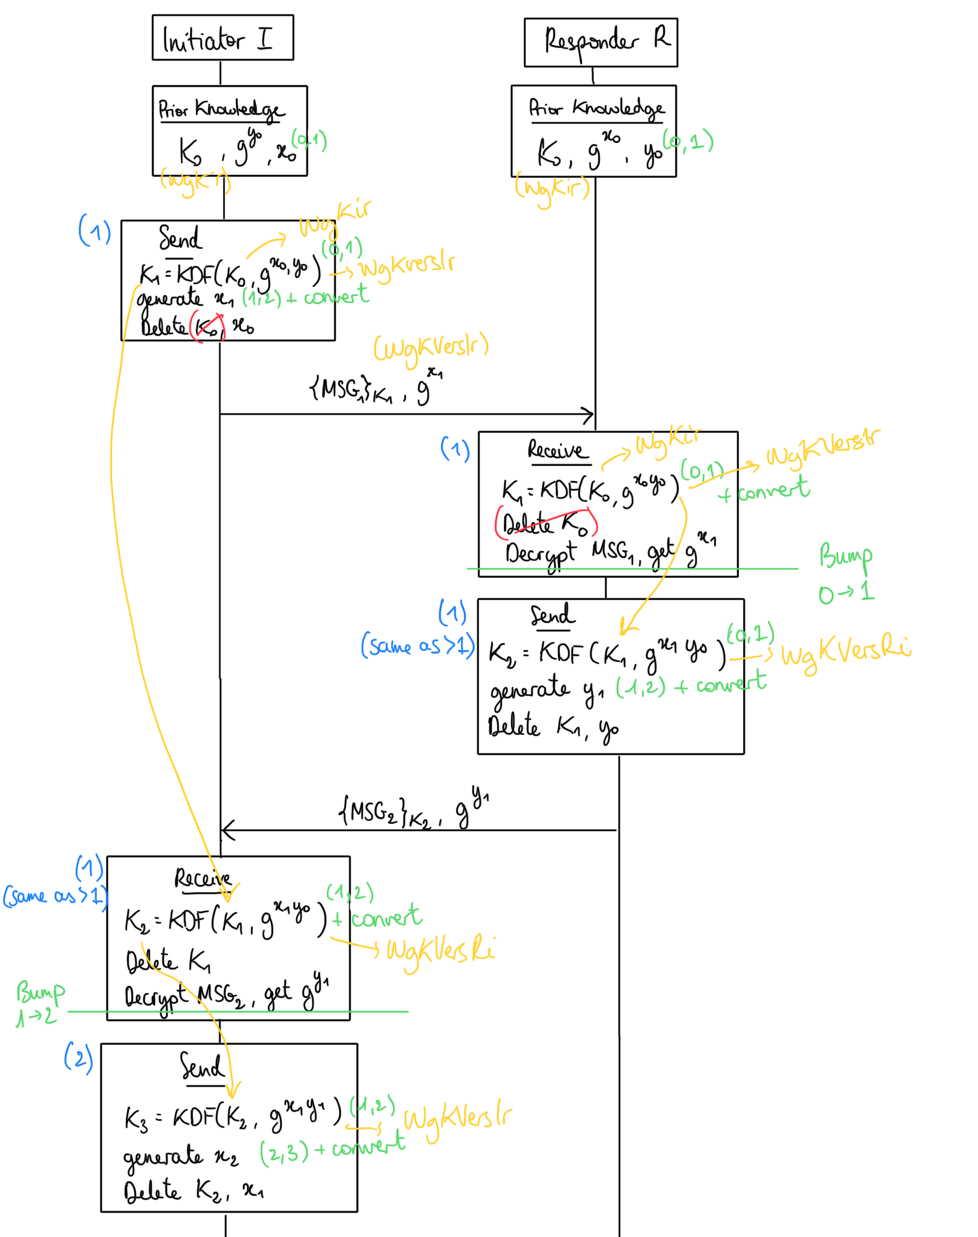
\includegraphics[width=0.9\textwidth]{figures/DH-ratchet-modified.png}
    \caption{Our \emph{ratcheting protocol}, a modified protocol based on the Diffie-Hellman Ratchet.}
    \label{fig:dh-ratchet-modified}
\end{figure}

\begin{figure}
    \centering
    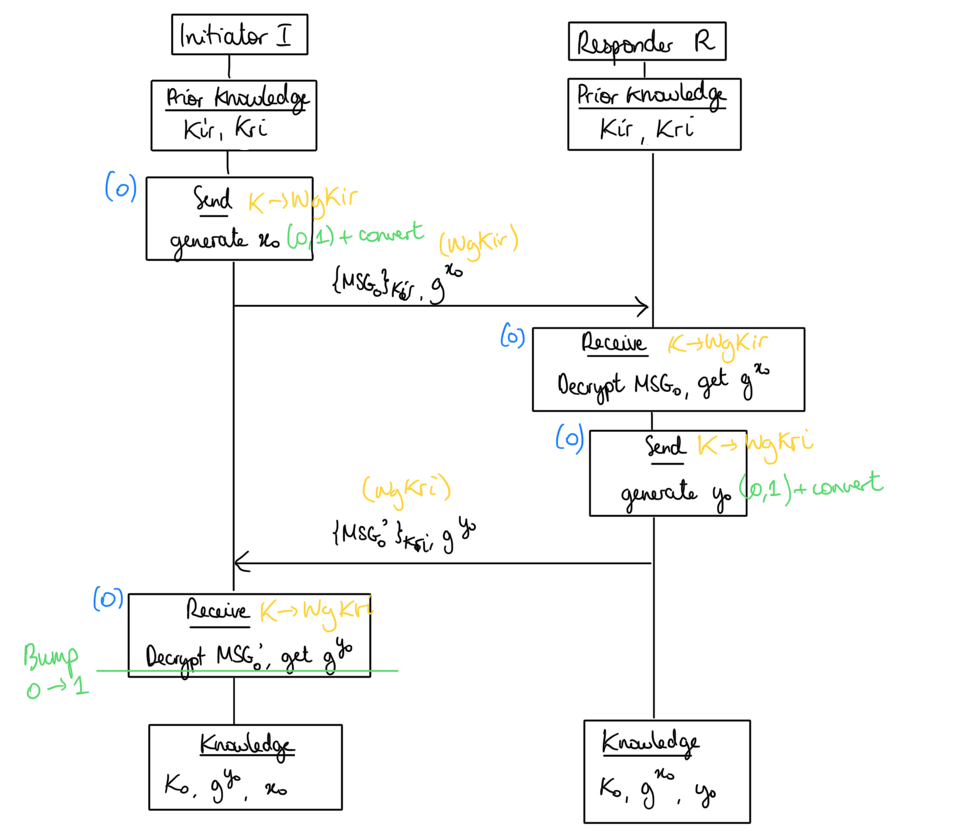
\includegraphics[width=0.9\textwidth]{figures/DH-ratchet-modified-first.png}
    \caption{First communication round after the handshake.}
    \label{fig:dh-ratchet-modified-first}
\end{figure}
\todo{Change the figures~\ref{fig:dh-ratchet-modified} and~\ref{fig:dh-ratchet-modified-first} to use cleaner ones, and modify the caption to explain the figures more in detail}

The intuition behind the ratcheting protocol is that we replicate the DH Ratchet protocol, but instead of using the just-received public key, we use the public key received in the previous message to compute the shared secret.
This first requires us to modify the prior knowledge of the participants. Now, in addition to the initial shared secret $K_0$, both participants need to know the other's DH public key and their (versioned) DH private key.
This is the purpose of the new first communication round shown in Figure~\ref{fig:dh-ratchet-modified-first}. 
The initiator first sends its public key $g^{x_0}$ to the responder, authenticated with the symmetric key $K_{IR}$ established by the handshake. Then, the responder replies with its authenticated public key $g^{y_0}$.

Coming back to the ratcheting protocol shown in Figure~\ref{fig:dh-ratchet-modified}, when computing the first shared secret $K_1$, the initiator uses its private key $x_0$, whose associated public key $g^{x_0}$ is already known by the responder, from the first communication round.
This was not the case in the DH Ratchet protocol.
The first message sent by the initiator to the responder is otherwise the same as in the DH Ratchet protocol and contains the initiator's new authenticated public key $g^{x_1}$ in addition to the encrypted message.
Upon reception of this message by the responder, instead of using the public key $g^{x_1}$ to compute the shared secret $K_1$, the responder uses the previous public key $g^{x_0}$ received in the first communication round.
This allows the responder to obtain $K_1$, decrypt the message, and obtain the associated message invariant containing information about the new public key $g^{x_1}$.
Then, $g^{x_1}$ is used just after by the responder to compute the next shared secret $K_2$, which is used to encrypt the next message sent to the initiator.
The same observations can be made upon reception of the second message by the initiator, and all subsequent messages. 
\todo{Depending on how precise the final Figure~\ref{fig:dh-ratchet-modified} is, I may need to explain the difference between the first message and the others: we do not delete the unversioned key $K_0$}

This ratcheting protocol is therefore simpler to verify than the DH Ratchet and aims to provide similar security properties.
Intuitively, forward secrecy still holds because past communication keys are deleted and cryptographically not retrievable from long-term secrets and current communication keys.

Additionally, we show that post-compromise security still holds.
Similarly to the original DH Ratchet protocol, we consider that the attacker compromised Alice's $K_n$ communication key \emph{after} her computation of the new $K_{n+1}$ key, and after she and her peer Bob have deleted their DH private key they used to compute $K_{n+1}$.
At this point, the attacker is unable to obtain $K_{n+1}$ because they cannot compute the associated DH shared secret.
Therefore, in this restricted compromise scenario, future communication remains secure.
The protocol is therefore healed and achieves post-compromise security.

% Additionally, we show that post-compromise security still holds.
% Considering a participant $p$ in a session $s$ and version $n$, we want to know how long the ratcheting protocol takes to heal. 
% If $p$ is deriving a new communication key $K_n$, we look at the consequences if the attacker had compromised $p$ or its peer $p'$ in the past.
% Recall that $p$ obtains their new key by computing $K_n := \text{KDF}(K_{n-1}, g^{xy})$, where $x$ and $y$ are private keys of $p$ and $p'$ respectively.
% For a past compromise to impact this key $K_n$, the attacker would need to know $K_{n-1}$ and either $x$ or $y$. Indeed, $g^x$ and $g^y$ have been publicly exchanged, so the attacker only needs to know one private key to compute the shared secret $g^{xy}$.
% Therefore, unless the attacker obtains $K_{n-1}$ and $x$ or $y$ between their creation and their deletion, the attacker cannot obtain $K_n$, meaning that the past compromise would not impact the future communication.
% This shows that our ratcheting protocol satisfies post-compromise security.

% For the sake of accuracy, we show that the difference between our protocol and the DH Ratchet protocol nevertheless has a slight impact on the exact property that our protocol satisfies.
% Note that at this point, the reasoning above is valid for both the DH Ratchet protocol and our ratcheting protocol.
% What differs between the two protocols is the amount of time between the creation of $K_{n-1}$, $x$ and $y$ and their deletion.
% Intuitively, the longer this amount of time is, the more likely it is that the attacker obtains $K_{n-1}$ and $x$ or $y$ to derive $K_n$ and compromise future communication.
% In our ratcheting protocol, we explained that $p$ uses the public key $g^y$ of $p'$ from the \emph{previous} communication round to compute the shared secret, instead of using the just-received one as in the DH Ratchet protocol.
% This means that after $p'$ creates $y$, they will first send a message where $g^y$ is given as associated data, and in the next round $p'$ will use $y$ to compute the shared secret of the communication key $K_n$ to send their next message.
% Because of this, $y$ still exists in the memory of $p'$ when they compute $K_n$ to encrypt the second message, whereas in the DH Ratchet protocol, $y$ would already be deleted and $K_n$ would be derived using a freshly generated private key.
% \todo{This is not the case in the current figure showing the DH Ratchet. It should be changed to show the deletion of $x$ and $y$ in the receive function.}
% In the end, our ratcheting protocol gives a slightly longer amount of time to the attacker to corrupt $p'$ to obtain $y$ before $K_n$ is computed, which would compromise all future communication.
% \todo{Is our protocol really weaker than the original?}
% Our ratcheting protocol therefore verifies post-compromise security with a marginally weaker security property than the DH Ratchet protocol.

% Recall that post-compromise security \emph{via state} considers that some secret data remains known only by the participants after a compromise.
% With the DH Ratchet protocol, we assumed that the attacker compromised Alice's $K_n$ key (and state) \emph{after} she derived $K_{n+1}$, and this assumption was enough to obtain post-compromise security (section~\ref{sec:security-properties}).
% However, this does not hold in this case.
% Suppose we have two participants Alice and Bob communicating, and that an attacker compromises Alice's state at the time when she computed $K_n$ after receiving a message.
% The attacker knows $K_n$, but also Alice's ephemeral private key $x_{n-1}$ and Bob's just-received public key $g^{y_{n-1}}$.
% The attacker can therefore compute $K_{n+1} = \text{KDF}(K_n, g^{x_{n-1}y_{n-1}})$ because it knows all the inputs of the KDF function, which was not the case with the DH Ratchet protocol.
% Unlike before, we have to assume that the attacker compromised Alice's $K_n$ key (and state) after she derived $K_{n+1}$ \emph{and} $K_{n+2}$.
% At this point, the attacker cannot obtain $K_{n+2}$ because they cannot have access to the new Diffie-Hellman shared secret.
% The protocol is therefore healed and achieves post-compromise security.

In the end, we have presented a full ratcheting protocol that draws its security properties from the frequent renewal of ephemeral keys. This protocol is mainly based on the Diffie-Hellman Ratchet protocol and has been slightly adapted to facilitate its verification, but achieves similar security properties.
We will now present how we implemented and verified this protocol using our methodology and its implementation in the Reusable Verification Library. 

\section{Implementation and verification}
\label{sec:implementation-and-verification}

This section explains how we implemented and verified the full ratcheting protocol presented in the previous section.
We started the implementation on top of the existing WireGuard implementation, which already implements the IKpsk2 handshake.
Our focus was on adapting the message transport phase to use the ratcheting protocol.
% The remaining work was to implement the first communication round and the ratcheting protocol.
In particular, the implementation work shed light on additional challenges related to the verification library. This section describes these challenges and how we solved them.

We start by explaining how we were able to model key ratcheting with our methodology.
Then, we present how we used usage constraints to distinguish between different types of messages and their associated message invariants.
Next, we focus on the first communication round and explain its specificities in terms of verification.
Afterward, we describe how we added verification annotations to comply with the requirements of our deletion mechanism when verifying the ratcheting protocol.
Finally, we explain how corruption is handled in the methodology and how we can integrate it into our verification annotations.

\subsection{Ratcheting using a key derivation function}
\label{sec:ratcheting-using-a-key-derivation-function}

In section~\ref{sec:creating-values-with-multiple-versions-for-ratcheting}, we explained how we designed our methodology to support key ratcheting, namely the derivation of a new key, versioned with a later version, from the previous one.
However, note that for now, we have not discussed the concrete specification and implementation of the ratcheting step. In particular, we have not discussed how we could obtain a $(v+1)$-versioned key from a $v$-versioned key.
% This is no coincidence, and we will explain why.

In practice, this ratcheting step is implemented by a key derivation function (KDF), taking the previous key as one of its inputs and returning the new key.
However, the precise KDF function used and the arguments it takes depend on the protocol. It is therefore not possible to provide a generic implementation of it in the library. This is why we have not discussed its implementation yet.
For our case study, the KDF function specification is given in Figure~\ref{lst:kdf-ratchet}.

\begin{figure}
    \begin{gobra}
trusted
requires versionPerm > 0 && acc(guard(currentVersion), versionPerm)
ensures  acc(receipt(res, currentVersion), versionPerm)
func ComputeKDFRatchet(k []byte, dhss []byte, ghost currentVersion
    uint32, ghost versionPerm perm @*/) (res []byte) {
    // ...
}
    \end{gobra}
    \caption{Specification of the trusted \texttt{ComputeKDFRatchet} function, taking the previous key \texttt{k} and Diffie-Hellman shared secret \texttt{dhss} as input, and whose body computes the KDF result \texttt{res}. This protocol-specific KDF implementation is not part of the library but is written by the developer as part of the protocol. Preconditions and postconditions that are not relevant to the deletion mechanism have been omitted.}
    \label{lst:kdf-ratchet}
\end{figure}

\texttt{ComputeKDFRatchet} is the concrete implementation of our KDF function, and as the underlying KDF computations come from a non-verified library, we have to trust it.
As with any function creating a versioned value in our methodology, it consumes some permission fraction of \texttt{guard} predicate and returns the same amount of \texttt{receipt} for the created value. This ensures the soundness of our deletion mechanism.

Now, we want to define the secrecy label of the resulting KDF.
The secrecy label of a term is defined by a function \texttt{GetLabel} in the library. It returns a static label depending on the properties of the term, or a label depending on the arguments of the term when the term is a function of other terms, e.g. the hash of a term.
But first, to define a secrecy label for the KDF output, we need the library to \emph{know} about our KDF. While we defined it in the protocol, the KDF function needs to be specified on the term level in the library. We define it as follows:
\begin{gobra}
func KDFRatchet(Term, Term) Term
\end{gobra}
We additionally specify some of its properties, like injectivity, through axioms written in the library.
To then bridge the gap between the protocol and the library definitions, we add to the protocol's \texttt{ComputeKDFRatchet} function a postcondition ensuring that the KDF result corresponds to the byte representation of the term resulting from applying the newly defined KDF function on the term level.

Now that the library knows about our KDF, we can define its secrecy label.
Intuitively, the only rule about the secrecy of a KDF output is that it is at most as secure as knowing all of its inputs. Indeed, if you know all the inputs of a KDF, you can compute its output.
However, the KDF output is not necessarily as secure as its inputs. For example, a \emph{hash} function behaves similarly to a KDF function and is generally used to obtain a public output from a secret input. 
Therefore, the secrecy label of the output of a KDF should be weaker or equal to the intersection of the secrecy labels of its inputs.

In our case, we chose to define the secrecy label of the KDF output term \texttt{newk~:= KDFRatchet(k, dhss)} as the secrecy label of the Diffie-Hellman shared secret \texttt{dhss} only.
% In our case, the output term \texttt{newk := KDFRatchet(k, dhss)} can have its secrecy label determined by the labels of the previous key \texttt{k} and the Diffie-Hellman shared secret \texttt{dhss}.
Indeed, considering $v$ the current session's version, because the input key $k$ is not $(v+1)$-versioned, it is easy to see that \texttt{newk} cannot obtain a secrecy label containing $(p,s,v+1)$ from \texttt{k} alone.
Instead, we show that the \texttt{dhss} term has to be $(v+1)$-versioned, therefore making \texttt{newk} $(v+1)$-versioned as well.
% which will then allow us to define the secrecy label of \texttt{newk} as being equal to the one of \texttt{dhss} only.

The shared secret $\texttt{dhss} = g^{xy}$ is obtained by exponentiating the public key $g^y$ of the other participant with our private key $x$.
As $x$ is our key, we get to define its secrecy label at creation. 
In our ratcheting protocol, $x$ is meant to be an ephemeral private used to derive the two next shared communication keys $K_n$ and $K_{n+1}$ (the first one for receiving and the other for sending, where $n$ is even and odd for Alice and Bob respectively), as shown in Figure~\ref{fig:dh-ratchet-modified}.
As we want to use $x$ to obtain a shared secret for the next round of communication, we make it readable in version $v+1$. Because any value also needs to be readable in the current version, $x$ is given the label $[(p,s,v),(p,s,v+1)]$, where $p$ and $s$ are the respective participant and session creating $x$.
From the message invariant, we obtain that $y$ is readable by the other participant $p'$. Because $p$ does not need to precisely know in which session and version $y$ is readable by $p'$, the message invariant only gives us the simplified secrecy label $[(p')]$ for $y$.
Then, the labeling rules defined in the existing library state that the secrecy label of the shared secret $g^{xy}$ is the union of $x$ and $y$'s secrecy labels, which is $[(p,s,v),(p,s,v+1),(p')]$.

This $(v+1)$-versioned secrecy label of \texttt{dhss} is exactly what we wanted for our \texttt{newk} term.
We define the labeling of our \texttt{KDFRatchet} term in the library by stating the following postcondition for the library's \texttt{GetLabel(term Term) (res SecrecyLabel)} function:
\begin{gobra}
ensures forall k, dhss Term ::
    term == KDFRatchet(k, dhss) ==> res == GetLabel(dhss)
\end{gobra}
Therefore, we have adapted our labeling rule and shown that following our ratcheting methodology, we can obtain a $(v+1)$-versioned key from a $v$-versioned key.
\todo{Make sure the code is on one page only}

\subsection{Usages and message invariants}
\label{sec:usages-and-message-invariants}

In section~\ref{sec:chosen-protocol}, we discussed how message invariants are crucial to the verification of our ratcheting protocol.
Recall that they are a property proven by the initiator upon AEAD encryption of a message, and obtained by the responder upon AEAD decryption of the received message.
It is important to note that each kind of message needs its message invariant.
In our case, we have several kinds of messages: a variety of messages used in the IKpsk2 handshake, the messages used in the first communication round, and the messages used in all subsequent rounds in the ratcheting protocol.
For the handshake messages, we have been able to fully reuse the existing message invariants from the WireGuard implementation, so we will not discuss them further.
This leaves us with two kinds of messages to consider.
% \todo{The truth is that in the end, I used the same message invariant for both types of messages. The following paragraphs however still seem necessary as they explain how I implemented new usages to use the right message invariants.}

Because of these different kinds of messages and their associated message invariants, we need to be able to distinguish them in the library.
To do so, the current implementation of the library, similarly to DY*~\cite{bhargavan2021text}, uses \emph{usage constraints}.
A usage is a way to annotate a term that should be used for a specific purpose.
For example in the case of our ratcheting protocol, we use usages to distinguish Diffie-Hellman private keys, public keys, shared secrets, and $K$ versioned communication keys.
A usage can initially be defined upon creation of a value. This is the case when creating a Diffie-Hellman private key.
But then, similarly to secrecy labels, usages of terms are obtained using a protocol-specific \texttt{GetUsage} function, which can return a usage depending on the arguments of the term when the term is a function of other terms.
For example, it is in this \texttt{GetUsage} function that we define that the exponentiation of the generator with a key of usage \emph{DH Private Key} has usage \emph{DH Public Key}.
Similarly, the exponentiation of a key of usage \emph{DH Public Key} with a key of usage \emph{DH Private Key} has usage \emph{DH Shared Secret}.

Coming back to the two kinds of messages in our ratcheting protocol that we need to distinguish, we use usages to do so.
Keys used in the first communication round already have a specific usage \texttt{KUsage} that they obtained at the end of the handshake.
For subsequent ratcheting keys, we extend the \texttt{GetUsage} function to return a specific usage \texttt{KVersUsage} for keys resulting from the \texttt{KDFRatchet(k, dhss)} function, where \texttt{k} is a key of usage \texttt{KUsage} or \texttt{KVersUsage}, and \texttt{dhss} has a \emph{DH Shared Secret} usage.

To be even more specific about the implementation, we found that it makes verification much easier to distinguish between messages coming from the initiator and messages coming from the responder, and to use slightly different message invariants for each.
Usage constraints were the natural way to do so, by defining a usage \texttt{KVersIrUsage} for keys used to encrypt a message sent from the initiator to the responder, and a usage \texttt{KVersRiUsage} for keys used to encrypt a message sent from the responder to the initiator (and similarly defining \texttt{KIrUsage} and \texttt{KRiUsage} for the first communication round).

Ultimately, using usage constraints, we can distinguish between different kinds of messages upon AEAD encryption and decryption, and identify messages coming from the initiator or the responder.
This simplifies the specification of message invariants because we can distinguish between messages and thus separately specify message invariants for kind of each message.

\subsection{First communication round}
\label{sec:first-communication-round}

As shown in Figure~\ref{fig:dh-ratchet-modified-first}, the first communication round is a little different from the other rounds.
Before it starts, the initiator and responder have a shared secret $K_0$ resulting from WireGuard's handshake.
The goal of this first round is to send authenticated public keys to each other so that they can start the ratcheting protocol.

The initial key $K_0$, coming from the WireGuard implementation, is not versioned so we will not be forced by the methodology to delete it. As it is only the first key, this will not have a big impact on the security properties of the protocol.
% However, outside the scope of this thesis, we could imagine implementing a versioned handshake resulting in a versioned $K_0$.
However, by also adapting the handshake and thus increasing verification efforts further, we could consider implementing a versioned handshake resulting in a versioned $K_0$.

But because $K_0$ is not versioned, we do not have a \texttt{receipt} for it.
This means that we cannot call the \texttt{DeleteSafely} function on it, as it requires such a receipt to consume it.
This has an impact on the second communication round, more particularly on the initiator's first send and the responder's first receive of the ratcheting protocol, shown in Figure~\ref{fig:dh-ratchet-modified}.
Indeed, these functions were the ones supposed to delete $K_0$ if it was versioned.
As they do not, the preconditions and postconditions of these functions may carry different amounts of guard and receipt permissions compared to all subsequent rounds.
This has to be kept in mind when working on verifying the protocol implementation in compliance with the requirements of the deletion mechanism.
This work is explained in the next subsection.

\subsection{Using the deletion mechanism}

In this section, we explain how we practically comply with the requirements of the deletion mechanism to verify the protocol implementation.
The first step in this process is to reason about the adequate times to increment the protocol session's version, at which point previous keys must be deleted.
This choice will directly impact the resulting security properties of the protocol.
Indeed, the more frequently we increment the session's version, the more we can reason about the temporal existence of keys with a fine granularity, which could lead to tighter security properties.
% Indeed, the more frequently we increment the session's version, the more frequently we delete ephemeral keys, and the stronger we expect the security properties to be.
Of course, there is no point in incrementing the version \emph{too} frequently.
If no data has been deleted between two versions, the last version increment is unnecessary and only results in added verification complexity without benefits.

In the case of our ratcheting protocol, we notice that with the notations of the Figure~\ref{fig:dh-ratchet-modified}, for $n>0$, the initiator's private key $x_n$ is used in the computation of the communication keys $K_{2n}$ and $K_{2n+1}$. We can obtain a similar result for the responder.
We also notice that we delete a key $K_{2n}$ just after we derive the next key $K_{2n+1}$.
As a first intuition, it would seem natural to increment the session's version just after we derive $K_{2n+1}$ so that we force the deletion of $K_{2n}$ at this point.
However, doing so is not possible.
Indeed, at each round, a participant first derives a receiving key $K_{2n}$ and then a sending key $K_{2n+1}$, using the \texttt{ComputeKDFRatchet} function.
While they use a different Diffie-Hellman shared secret to derive each key, both shared secrets use the same private key $x_n$.
Recalling the explanations about the labeling of the KDF result given in section~\ref{sec:ratcheting-using-a-key-derivation-function}, we see that the secrecy label of $x_{n}$ defines the secrecy label of the KDF results $K_{2n}$ and $K_{2n+1}$ for the calling participant.
Because the part of the secrecy label about the other participant $p'$ is always the same, $(p')$, the secrecy label of $K_{2n}$ and $K_{2n+1}$ is the same.
% This means that for a participant $p$ in session $s$ calling the \texttt{ComputeKDFRatchet} function to derive $K_n$ and then $K_{n+1}$, the part of the secrecy label specifying their permissions is the same for both keys.
Therefore, as we give $x_{n}$ the label $[(p,s,n),(p,s,n+1)]$, the secrecy label of $K_{2n}$ and $K_{2n+1}$ is $[(p,s,n),(p,s,n+1),(p')]$.
Because of this, forcing the deletion of $K_{2n}$ after deriving $K_{2n+1}$ would require to increment the session's version to $n+2$, which would also force the deletion of $K_{2n+1}$.

Therefore, we have to use a coarser granularity for our versioning.
We saw that the secrecy label of a $K_{2n}$ communication key is fully determined by the label given to the Diffie-Hellman private key $x_{n}$ used to derive it.
We would then achieve the best possible granularity by incrementing the session's version between the computation of two private keys $x_{n}$ and $x_{n+1}$.
This way, supposing having $x_{n}$ with secrecy label $[(p,s,n),(p,s,n+1)]$, we aim to obtain $x_{n+1}$ with secrecy label $[(p,s,n+1),(p,s,n+2)]$.
Let's increment the session's version at the end of the receive function, before calling the send function, and observe what happens.

We look at the initiator $p$, supposing they are in session $s$ and version $n$, at the beginning of their receive function. We suppose having a private key $x_{n}$ with secrecy label $[(p,s,n),(p,s,n+1)]$, and a previous communication key $K_{2n-1}$ with secrecy label $[(p,s,n-1),(p,s,n),(p')]$.
As we explained, we first compute the key $K_{2n}$ that has a secrecy label $[(p,s,n),(p,s,n+1),(p')]$.
We can then delete $K_{2n-1}$ as it is not needed anymore.
Next, we increment the session's version to $n+1$.
Doing so, the methodology \emph{forces} us to delete $K_{2n-1}$ because it does not flow to version $n+1$.
We then decrypt the received message using $K_{2n}$ and the receive function ends.
Now, in the send function, we start by deriving the next communication key $K_{2n+1}$, which has a secrecy label $[(p,s,n),(p,s,n+1),(p')]$, like $K_{2n}$.
Next, we delete $K_{2n}$ and $x_{n}$, as they are not needed anymore.
We then compute the next private key $x_{n+1}$, choosing its secrecy label to be $[(p,s,n+1),(p,s,n+2)]$.
We finish by sending our message encrypted with $K_{2n+1}$, and the send function ends.
In this case, we were not forced yet to delete $K_{2n}$ and $x_{n}$, because we are still in version $n+1$.
However, we will be forced to delete these two values at the end of the next receive, when we will increment the session's version to $n+2$.
This granularity should be sufficient to later express our security properties.

Now that we have decided on the granularity of our versioning, we simply follow the requirements of the deletion mechanism that we described in section~\ref{sec:extension-of-the-library}.
These requirements mostly consist of specifying the “correct” amount of \texttt{guard} and \texttt{receipt} permissions in function calls. 
Additionally, recall the \texttt{ConvertToNextVersion} function introduced in section~\ref{sec:conversion-function}.
The developer will have to convert values labeled with multiple versions (private keys $x$ and communication keys $K$) when necessary, to keep using them in the next session's version.

\begin{figure}
    \begin{gobra}
requires iter == 0 ==> 
    acc(guard(v), p) && acc(guardNext(v+1), p)
requires iter == 1 ==> 
    acc(guard(v), 2*p) && acc(guardNext(v+1), p) &&
    acc(receipt(privKey, v), p)
requires iter > 1  ==>
    acc(guard(v), 2*p) && acc(guardNext(v+1), p) &&
    acc(receipt(privKey, v), p) && acc(receipt(K, v), p)
ensures iter == 0 ==>
    acc(guard(v), p) && acc(receipt(newPrivKey, v+1), p)
ensures iter == 1 ==>
    acc(guard(v), 2*p) && acc(receipt(newK, v), p) &&
    acc(receipt(newPrivKey, v+1), p)
ensures iter > 1  ==>
    acc(guard(v), 3*p) && acc(receipt(newK, v), p) &&
    acc(receipt(newPrivKey, v+1), p)
func SendMessage(K []byte, privKey []byte, iter int, ghost v uint32,
    ghost p perm) (newK []byte, newPrivKey []byte) {
    // ...
}
    \end{gobra}
    \caption{Specification of the function \texttt{SendMessage} that sends a message in the ratcheting protocol. Preconditions, postconditions and arguments that are not relevant to the deletion mechanism have been omitted.}
    \label{lst:send-message}
\end{figure}

To give a final intuition about the actual reasoning that the developer has to do to comply with the deletion mechanism, we give in Figure~\ref{lst:send-message} the preconditions and postconditions related to the \texttt{guard} and \texttt{receipt} predicates of the initiator's send function.
The case \texttt{iter == 0} corresponds to the send operation in the first communication round. Here, a fraction of \texttt{guard(v)}, where $v$ is the current version, is necessary to create the new Diffie-Hellman private key \texttt{newPrivKey}. As it is created with a label $[(p,s,v),(p,s,v+1)]$, we then convert it to the next version $v+1$. This consumes the fraction of \texttt{guard(v+1)} and returns both a fraction of \texttt{receipt(newPrivKey, v+1)} and a fraction of \texttt{guard(v)}.
The case \texttt{iter == 1} corresponds to the second send operation of the initiator, so to the first send operation of the ratcheting protocol. Compared to previously, we additionally need another \texttt{guard(v)} fraction to compute the initial KDF, which in turn returns a \texttt{receipt(newK, v)} fraction. And we delete the previous private key, consuming the \texttt{receipt(privKey, v)} fraction and returning a \texttt{guard(v)} fraction.
Finally, the case \texttt{iter > 1} is the same as before but with the additional deletion of the previous communication key, consuming the \texttt{receipt(K, v)} fraction and returning an additional \texttt{guard(v)} fraction.

\subsection{Corruption}

In the existing methodology, an attacker can corrupt a participant's memory and obtain the stored secrets.
The methodology distinguishes between the corruption of a participant, leaking all of their long-term secrets, and the corruption of a particular session, leaking all of the secrets of the session in addition to the long-term secrets.
With our extended methodology, we add the case of corrupting a version, leaking all of the ephemeral secrets of the version in addition to the session secrets and the long-term secrets.
Corruption is a crucial notion to consider when verifying a protocol, as we need it to express strong security properties. In particular, certain security properties hold even under some cases of corruption.
For example, post-compromise security states that a key remains secret even if the attacker has corrupted certain versions in the past.

In the Reusable Verification Library, corruption is modeled upon receiving and decrypting an AEAD encrypted message. 
Recall from section~\ref{sec:chosen-protocol} that upon decryption, we obtain a message invariant containing properties about the message that were proved by the sender, unless the attacker performed the encryption.
In the latter case, the attacker must have computed the encryption and accessed the encryption key and message, i.e. the secrecy labels of the encryption key and the message must flow to \emph{Public}.
% To be precise, we either obtain this message invariant, or we do not and we thus learn that the message comes from the attacker.
% In the latter case, corruption is modeled by learning that the message and its encryption key are known to the attacker, i.e. that their secrecy labels flow to \emph{Public}.

Coming back to our ratcheting protocol, we have seen in the previous section that an ephemeral communication key has a secrecy label of the form $[(p,s,v),(p,s,v+1),(p')]$, where $v$ is the current version of session $s$.
If we learn that the message came from the attacker and thus the secrecy label of the encryption key flows to \emph{Public}, we learn that either version $(p,s,v)$, or version $(p,s,v+1)$, or the long-term secrets of participant $p'$ must have been corrupted\footnote{Which is also the case when any session or any version of a session of $p'$ has been corrupted.}.
Indeed, corrupting any of these is the only way for the attacker to obtain the communication key, as proven in the secrecy lemma of the existing methodology.

In practice, this results in case distinctions while verifying our protocol implementation.
Upon receiving and decrypting a message, we have to consider the case where we receive the message invariant and the case where we know that corruption occurred.
In the second case, not obtaining the message invariant means that we learn nothing about the associated data of the encrypted message. In our ratcheting protocol, we do not learn that the associated data is an exponential of the form $g^y$, with a \emph{DH Public Key} usage, where $y$ is a private key readable by the other participant.

This has an impact on other verification annotations of the protocol because these case distinctions propagate to other preconditions and postconditions.
For example, the receive function of the protocol implementation can return information about the received public key only when the message invariant is obtained, but not in case of corruption.
And the subsequent send operation is supposed to compute a shared secret using the received public key, to then derive the next communication key.
The preconditions of these functions must be satisfied in both cases, whether we obtained the message invariant or not.
In practice, we make the receive function of the protocol return a ghost boolean parameter \texttt{newCorrupted} to inform the caller whether corruption must have occurred or not.
We additionally introduce a ghost boolean parameter \texttt{corrupted} as input of the receive and send functions of the protocol, and we use it to express different preconditions and postconditions, and call different lemmas depending on the particular case we are in.

% \todo{Maybe sum up what we have done/implemented/verified yet?}
This work of integrating corruption in the verification annotations of the protocol implementation turned out to be a tricky and time-consuming task.
In the scope of this thesis, we were not able to fully complete it.
We discuss in detail in the next section the remaining work to be done to fully integrate corruption into our proof, to complete the verification of the strong security properties of our ratcheting protocol.

\section{Remaining work}
\label{sec:remaining-work}
% Prove CanAeadEncrypt in the corrupted case
%   Change usage rule for KVers
%   Handle secrecy label and corruption
% Prove K convert in the corrupted case
% Prove security properties

In this section, we detail how one could finish the verification of our ratcheting protocol.
We list the missing parts of the verification work and we provide a clear path to complete them.

First, we need to satisfy the AEAD encryption requirements in the corrupted case.
Upon encryption, the current methodology requires us among others to prove that the encryption key has an appropriate usage.
A usage is defined as “appropriate” for AEAD encryption by the developer in the \texttt{GetUsage} function.
In our case, the usages \texttt{KVersIrUsage}, \texttt{KVersRiUsage}, \texttt{KVersIrUsage} and \texttt{KVersRiUsage} defined in section~\ref{sec:usages-and-message-invariants} are defined as being appropriate for AEAD encryption.
However, in the corrupted case, we do not know the usage of the received associated data, which we expect to be the other participant's public key.
The current usage rules prevent us from proving that the shared secret obtained from this public key and our private key has a \emph{DH Shared Secret} usage.
Hence, we cannot show that the encryption key obtained with \texttt{KDFRatchet} from the previous key and this shared secret has an appropriate usage for AEAD encryption.
To solve this, we suggest changing the protocol-specific usage rules defined in \texttt{GetUsage} to make the usage of \texttt{KDFRatchet}'s output independent of the usage of its shared secret input.
Thus, we would be able to prove that the encryption key has an appropriate usage for AEAD encryption even in the corrupted case.

To satisfy the AEAD encryption preconditions, we additionally have to show that there exists a label that flows to the encryption key and to which the secrecy label of the message flows.
In the non-corrupted case, we use the secrecy label $[(p,s,v),(p,s,v+1),(p')]$ of the encryption key, to which the message secrecy label $[(p,s),(p')]$ flows.
In case of corruption, the secrecy label of the encryption key is harder to determine because we know nothing about the received associated data and we cannot assume that it is the other participant's public key.
We have to make a disjunction on what the received associated data could be to compute the secrecy label of the encryption key in each case.
By doing so, we can show that in all cases, the secrecy label of the encryption key flows to the label of the DH secret key used to compute it, which is $[(p,s,v),(p,s,v+1)]$. As the secrecy label of the message flows to this label, we satisfy the AEAD encryption precondition.

Overall, verifying our protocol implementation in case of corruption will require us to make several case distinctions and to call additional lemmas to complete each case's proof.
While time-consuming, we are confident that it is completely doable.

Next, the last part of the verification work is to prove the security properties of our ratcheting protocol.
All the verification annotations that we have introduced before, which model concepts like versions and corruption, were added to be able to express security properties.
Suppose a participant $p$ executes the ratcheting protocol in session $s$ and version $v$, with a peer participant $p'$.
We have shown that the current communication key $K_n$ has a secrecy label of the type $[(p,s,v),(p,s,v+1),(p')]$.
$K_n$ remains secret unless the attacker compromises the version $v$ or $v+1$ of the session $s$, or the other participant $p'$.

However, our secrecy property is currently weaker than it could be, as the secrecy label of $K_n$ contains $p'$, which expresses that $K_n$ can be obtained by the attacker if they compromise $p'$ at any time.
This property could be strengthened, as we can intuitively see that $K_n$ is also available in only two versions of a session $s'$ of $p'$.
We leave it to future work to show that, when $p$ is the initiator and for $n>0$, the secrecy label of $K_{2n}$ can be strengthened to $[(p,s,n),(p,s,n+1),(p',s',n-1),(p',s',n)]$ and the secrecy label of $K_{2n+1}$ can be strengthened to $[(p,s,n),(p,s,n+1),(p',s',n),(p',s',n+1)]$.
Showing this requires tightening the message invariant that we initially introduced in section~\ref{sec:ratcheting-using-a-key-derivation-function}. 

% This means that $K_n$ remains secret even if the attacker compromises a version $v_{corrupted} \in \mathbb{N} \setminus \{v, v+1\}$ of the session $s$ of participant $p$, or a version $v'_{corrupted} \in \mathbb{N} \setminus \{v', v'+1\}$ of the session $s'$ of participant $p'$.
Then, we can express that the key $K_{2n+1}$ remains secret unless the previous key $K_{2n}$ was made public before $K_{2n+1}$ was computed, or unless the attacker compromises a version $n$ or $n+1$ of the session $s$ of participant $p$ or of the session $s'$ of participant $p'$.
Indeed, if the attacker compromises $K_{2n}$ before $K_{2n+1}$ is computed, they could impersonate a protocol participant and eventually obtain $K_{2n+1}$.
Similarly, we express that a key $K_{2n}$ remains secret unless the previous key $K_{2n-1}$ was made public before $K_{2n}$ was computed, or unless the attacker compromises a version $n$ or $n+1$ of the session $s$ of participant $p$ or a version $n-1$ or $n$ of the session $s'$ of participant $p'$.
Overall, these secrecy properties express both forward secrecy and post-compromise security for our ratcheting protocol.

To sum up, we have shown the path to complete the verification of our protocol's security properties.
This will require some modifications to existing annotations, including strengthening the message invariant and probably writing additional lemmas. 

\section{Results}
\label{sec:results}

We finish this case study by reporting some quantitative results about the verification of our full ratcheting protocol.
Figure~\ref{fig:results} provides the number of lines of code (LOC), the number of lines of specification (LOS) and the verification time for the implementations of the full ratcheting protocol and the original WireGuard.
The number of lines of specification does not count the lines of the Reusable Verification Library, and the verification time does not include the time to verify the library.
This is justified because the library is protocol-independent and can be verified once and for all.

Our full ratcheting protocol is composed of 759 lines of code and 6167 lines of specification, which is around 8.1 times more specification than code.
However, note that the verification of the full ratcheting protocol is not complete yet and we thus expect a slightly higher ratio of specification to code once it is.
In comparison, the original WireGuard implementation is composed of around 9.8 times more specification than code, but corruption has been fully integrated into its specification and its security properties have been verified.

The verification time of our full ratcheting protocol is 669.5 seconds, which is around 1.5 times more than the verification time of the original WireGuard implementation.
This can be explained in part because our full ratcheting protocol contains additional specifications related to our deletion mechanism, which is not present in the original WireGuard implementation.
% the fact that the WireGuard specification makes better use of modularity, i.e. is composed of more functions, each with a smaller specification.
% We are confident that one could improve the modularity of our specification and thus reduce its verification time.


\begin{figure}
    \centering
    \begin{tabular}{@{}llll@{}}
        \toprule
        Protocol                 & LOC & LOS  & Verification time {[}s{]} \\ \midrule
        Full ratcheting protocol & 759 & 6167 & 669.5                     \\
        WireGuard                & 550 & 5411 & 441.8                     \\
        \bottomrule
    \end{tabular}
    \caption{Lines of code (LOC), lines of specification (LOS) and verification time for the implementations in Gobra of the full ratcheting protocol and the original WireGuard. The numbers for the latter are provided for reference because the full ratcheting protocol builds on top of the original WireGuard protocol. We have measured the verification time by averaging over 3 runs on a 2020 Apple MacBook Pro with a 4-core Intel Core i5 processor and 16 GB of RAM.}
    \label{fig:results}
\end{figure}




\chapter{Conclusion}
\label{chap:conclusion}


\appendix

% \chapter{Dummy Appendix}

You can defer lengthy calculations that would otherwise only interrupt
the flow of your thesis to an appendix.


\backmatter

\bibliographystyle{plain}
\bibliography{bibliography}

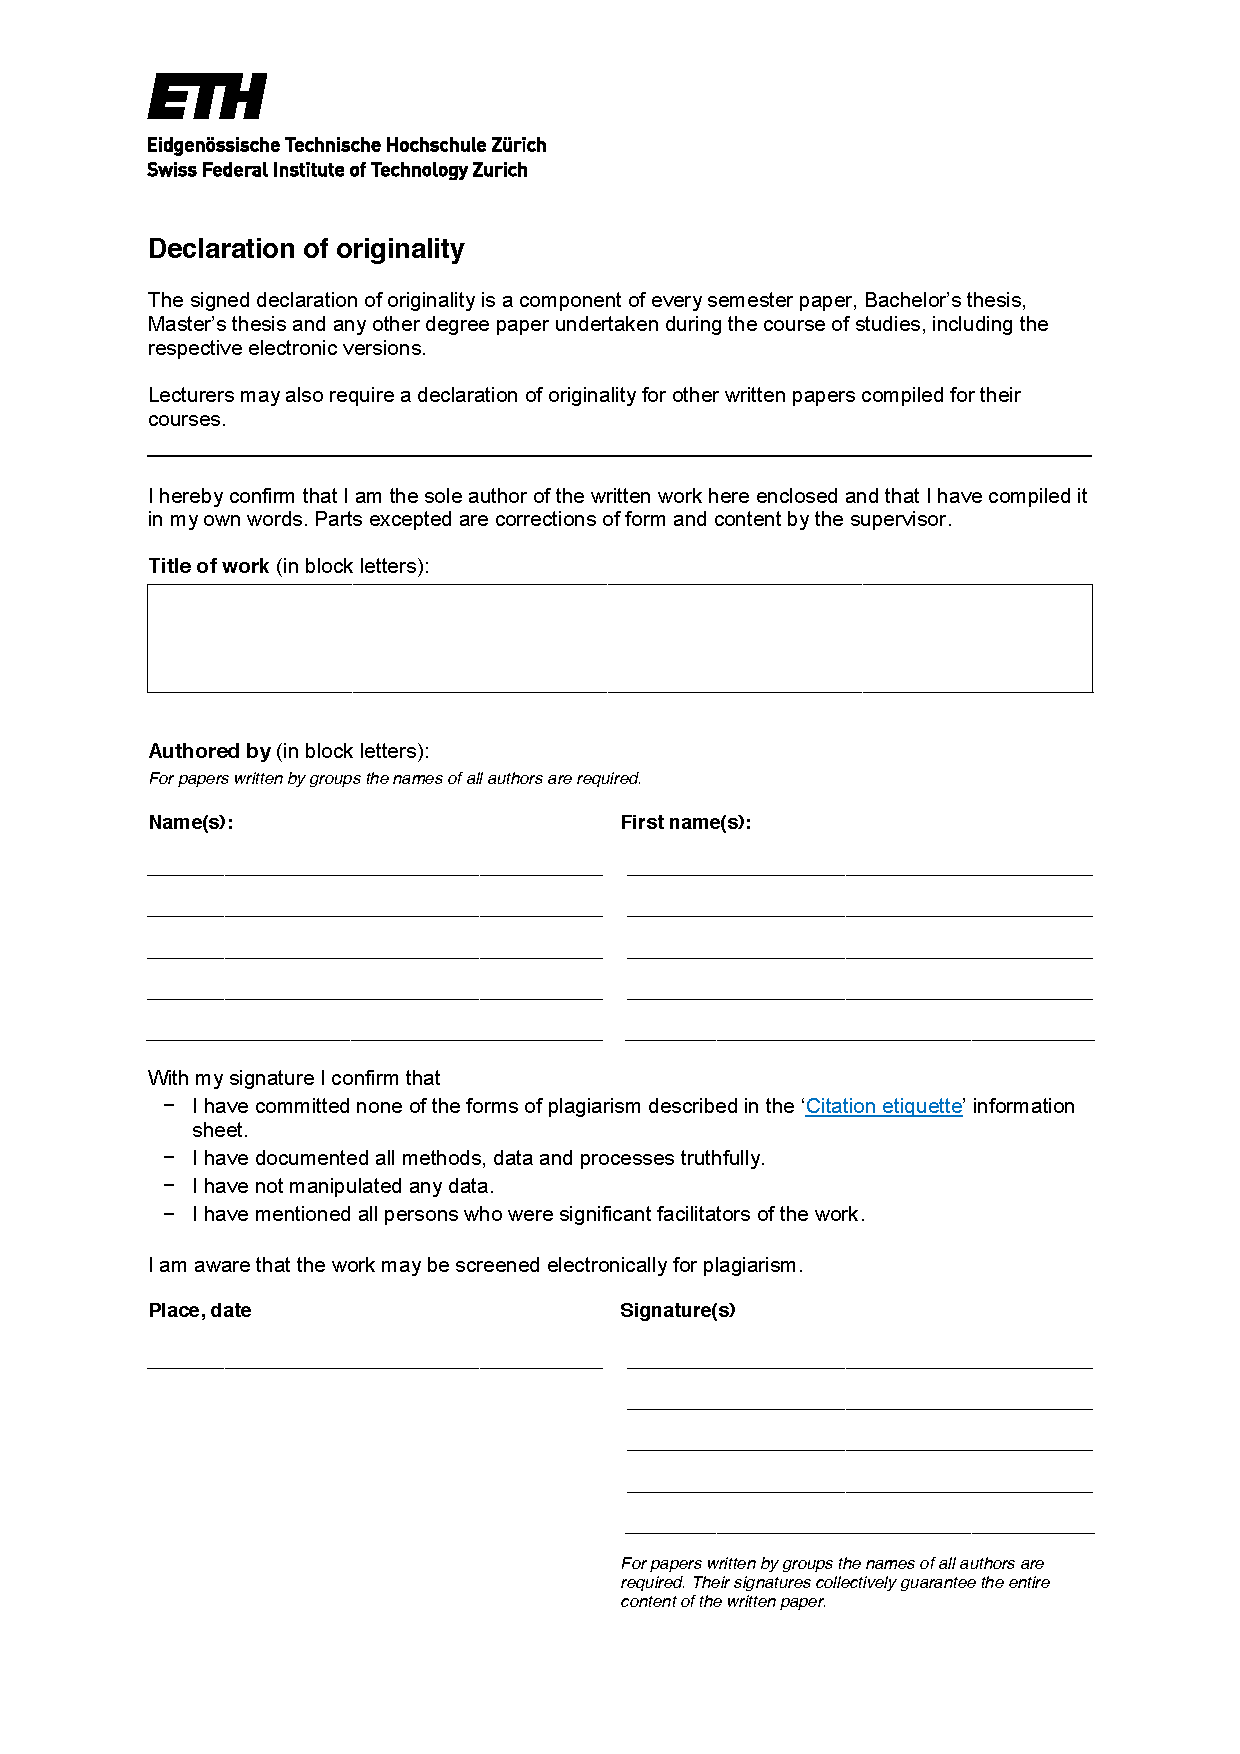
\includepdf[pages={-}]{declaration-originality.pdf}

\end{document}
